\documentclass{ctexart}
\usepackage{amsmath,amsthm,amssymb}
\usepackage{graphicx,subcaption}
\usepackage{algorithm,algpseudocode}
\usepackage{glsc}

\begin{document}

\title{基于Group LASSO的稀疏子空间聚类}
\author{张航}
\maketitle

\section{简介}

子空间聚类问题来自于很多实际的应用,包括运动轨迹分离~\cite{costeira1998motion_seg},
人脸识别~\cite{basri2003lambertianface},网络跳点计数~\cite{eriksson2011high_rankMC},
电影评分~\cite{zhang2012RecSys} 以及社交图谱~\cite{xu2011graphclustering}。
这些应用产生的高维数据通常可以看作是从多个混合的低维线性子空间的采样(如图\ref{fig:Union_of_sub_model}所示)。
子空间聚类就是在不知道类别信息的情况下,将这些数据按照它们原本所属的子空间重新聚合,
并且恢复出数据中隐含的子空间结构。
对应于上面所述的应用,子空间聚类能根据运动轨迹分离刚体,判断哪些面部照片来自同一个人,哪些网络
节点属于一个子网,给出观影兴趣相似的用户以及发现社交网络中隐含的人际关系。

\begin{figure}
  \centering
  % Requires \usepackage{graphicx}
  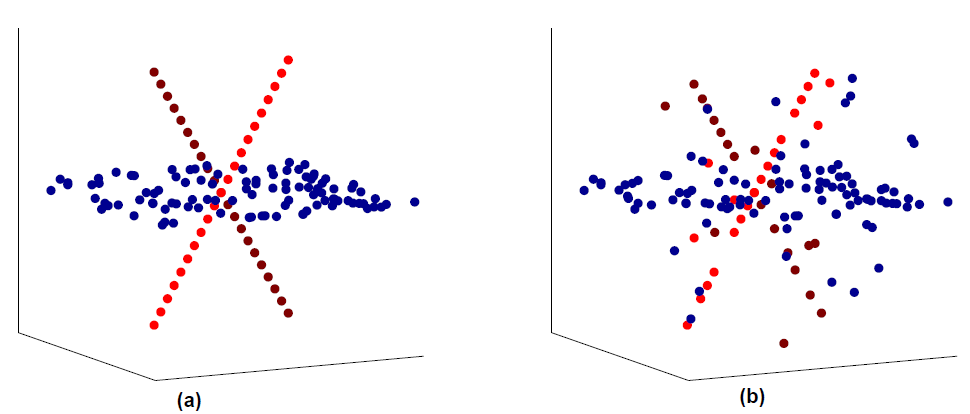
\includegraphics[width=0.8\linewidth]{pics/Union_of_Subspace.png}\\
  \caption{采样于三个子空间的无噪音 (a) 和有噪音 (b) 数据}\label{fig:Union_of_sub_model}
\end{figure}

过去十年,很多人关注子空间聚类问题,并且提出了许多算法,包括 Expectation-Maximization 类型的局部优化算法,
比如 K-plane~\cite{bradley2000k-plane} 和 Q-flat~\cite{tseng2000qflat},代数方法,比如
广义主成分分析(Generalized Principal Component Analysis)~\cite{vidal2005gpca},
矩阵分解方法~\cite{costeira1998motion_seg,costeira2000multibody_factorization},基于谱聚类的方法
~\cite{lauer2009spectral,chen2009spectral},自底向上的局部采样方法~\cite{yan2006LSA,rao2008motion},
以及基于凸优化的方法,比如低秩表示(Low Rank Representation)~\cite{liu2010lrr_icml,liu2013LRR}
和稀疏子空间聚类(Sparse Subspace Clustering)~\cite{elhamifar2009ssc,elhamifar2012ssc_journal}。
这些算法中,SSC是最优秀的之一,尤其当数据有噪音时,表现地相对稳健和鲁棒,例如在运动分割领域的
Hopkins155~\cite{tron2007benchmark,elhamifar2009ssc}测试集上,SSC是目前公认的表现最好的算法,
并且当类别增多时,它表现得比 LRR 更好~\cite{elhamifar2012ssc_journal}。

SSC算法的关键是将每个数据点用其他点线性表示,由于每个点都在一个低维子空间中,则一定存在一个相对稀疏的表示,
只用到同一个子空间中的点。如果把系数大小看作两个点的连接权重,我们可以得到一个无向图,再对这个图进行谱聚类,
即可将不同子空间的点分开。如果用第~\ref{sec:prob_setup}节中的符号描述,那么无噪音和有噪音的 SSC 分别求解
\begin{align*}
  \min_{c_i} \|c_i\|_1\quad s.t.\quad X_i=X_{\{i\}^c}c_i, \\
  \min_{c_i} \|c_i\|_1+\frac{\lambda}{2}\|X_i-X_{\{i\}^c}c_i\|^2,
\end{align*}
$X_i$ 表示数据矩阵的第$i$ 列, $c_i$ 是$X_i$ 用其他所有点表示的系数,我们希望其非零元素对应的数据点都和 $x_i$ 在同一个子空间。
对于仿射子空间,SSC 同样适用,只需要加上 $c_i = i$的限制。

然而,在 SSC 中,我们每次只考虑一个点相对于其他点的表示,
比较容易受到噪音和异常点的干扰。如果我们预先知道点$A,B,C$
属于同一类,然后寻找其他几个点能同时表示$A,B,C$,这无疑比
单独考虑$A$ 或 $B$ 或 $C$ 更稳健。另一方面,在SSC 模型中,
我们只是要求稀疏尽量稀疏,如此产生的邻接矩阵,不一定能在
接下来的谱聚类中有比较好的可分性。如果我们能让表示向量的非零元
集中在某些位置,那么邻接矩阵将具有更好的结构(具体可见第\ref{sec:experiments}节)

基于上面的考虑,本文提出了一种新的子空间聚类方法,它的核心内容有两步:
首先根据点的空间信息,将某些很可能是一类的点聚在一起。然后我们在剩余的
点中,寻找能同时表示它们的点,进而构造邻接矩阵。
coefficients of these exemplar data points are likely to be
seen significant across different representations for many
data points. But on the other hand, the representation for
each data point still needs to respect the sparse subspace
assumption. 事实上,压缩感知中的 joint sparse 模型[1]  [17] 很好地满足了我们的需求。
另一方面

Effort has been made to explain the practical success of SSC by analyzing the noiseless version. \cite{elhamifar2010ssc_icassp} show that under certain conditions, \emph{disjoint} subspaces (i.e., they are not overlapping) can be exactly recovered.
%Similar guarantee, under stronger ``independent subspace'' condition, was provided for LRR in a much earlier analysis\cite{kanatani2001motion}.
A recent geometric analysis of SSC~\cite{soltanolkotabi2011geometric} broadens the scope of the results significantly to the case when subspaces can be overlapping. However, while these analyses advanced our understanding of SSC, one common drawback
is that data points are assumed to be lying {\em exactly} on the subspaces. This assumption can hardly be satisfied in practice. For example, motion trajectories data are only {\em approximately} of rank-4 due to perspective distortion of camera, tracking errors and pixel quantization~\cite{costeira1998motion_seg}; similary, face images are   not precisely of rank-9 since human faces are at best {\em approximated} by a convex body~\cite{basri2003lambertianface}.

In this paper, we address this problem and provide a theoretical analysis of SSC with noisy or corrupted data. Our main result shows that a modified version of SSC (see Eq. \eqref{eq:Lasso}) succeeds when the magnitude of noise does not exceed a threshold determined by a geometric gap between the \emph{inradius} and the \emph{subspace incoherence} (see below for precise definitions). This complements the result of \cite{soltanolkotabi2011geometric} that shows the same geometric gap determines whether SSC succeeds for the noiseless case. Indeed,  when the noise vanishes, our results reduce to the noiseless case results of \cite{soltanolkotabi2011geometric}.

While our analysis is based upon the geometric analysis of \cite{soltanolkotabi2011geometric}, the analysis is more involved: In SSC, sample points are used as the dictionary for sparse recovery, and therefore noisy SSC requires analyzing a noisy dictionary.
%This is a hard problem and we are not aware of any previous study that proposed guarantee in the case of noisy dictionary except \cite{loh2012high} in the high-dimensional regression problem.
We also remark that our results on noisy SSC are {\em exact}, i.e., as long as the noise magnitude is smaller than a threshold, the recovered subspace clusters are {\em correct}.
This is in sharp contrast to the majority of previous work on structure recovery for noisy data where stability/perturbation bounds are given~--~i.e., the obtained solution is {\em approximately} correct, and the approximation gap goes to zero only when the noise diminishes.

Lastly, we remark that an independently developed work \cite{soltanolkotabi2013robust} analyzed the same algorithm {\em under a statistical model} that generates the data. In contrast, our main results focus on the cases when the data are deterministic. Moreover, when we specialize our general result to the same statistical model, we show that we can handle a significantly larger amount of noise under certain regimes.

%{\color{red}[Is this sentence too strong, since ours is stronger in some situations, and weaker in others]}. We will describe the differences in the next section.


%Then in Section~\ref{sec:ADMM_matrix-LASSO-SSC} we derive a fast numerical solver for the matrix version of our algorithm.

\section{Related works}\label{sec:RelatedWorks}
In this section, we review  previous and ongoing theoretical studies on the problem of subspace clustering.

\subsection{Nominal performance guarantee for noiseless data}
Most previous analyses concern about the nominal performance of a particular subspace clustering algorithm with noiseless data. The focus is to relax the assumptions on the underlying subspaces and data generation.

A number of methods have been shown working under the \emph{independent subspace} assumption including the early factorization-based methods \cite{costeira1998motion_seg,kanatani2001motion}, LRR~\cite{liu2010lrr_icml} and the initial guarantee of SSC~\cite{elhamifar2009ssc}. Recall that the data points are drawn from a union of subspaces, the \emph{independent subspace } assumption requires each subspace to be linearly independent to the {\em span} of all other subspaces. Equivalently, this assumption requires the sum of each subspace's dimension to be equal to the dimension of the span of all subspaces. For example, in a two dimensional plane, one can only have 2 independent lines. If there are three lines intersecting at the origin, even if each pair of the lines are independent, they are not considered independent as a whole.

\emph{Disjoint subspace} assumption only requires pairwise linear independence, and hence is more meaningful in practice. To the best of our knowledge, only GPCA~\cite{vidal2005gpca} and SSC~\cite{elhamifar2010ssc_icassp,elhamifar2012ssc_journal} have been shown to provably handle the data under \emph{disjoint subspace} assumption. GPCA however is not a polynomial time algorithm. Its computational complexity increases exponentially with respect to the number and dimension of the subspaces.

\cite{soltanolkotabi2011geometric} developed a geometric analysis that further extends the performance guarantee of SSC, and in particular it covers some cases when the underlying subspaces are slightly \emph{overlapping}, meaning that two subspaces can even share a basis. The analysis reveals that the success of SSC relies on the difference of two geometric quantities (inradius $r$ and incoherence $\mu$) to be greater than $0$, which leads to by far the most general and strongest theoretical guarantee for noiseless SSC. A summary of these assumptions on the subspaces and their formal definition are given in Table~\ref{tab:subspaces}.
\begin{table}
  \centering
\begin{tabular}{|l|c|}
  \hline
  % after \\: \hline or \cline{col1-col2} \cline{col3-col4} ...
  Independent Subspaces & $\dim\left[\cS_1\otimes...\otimes \cS_L\right] = \sum_{\ell=1}^L \dim\left[\cS_\ell\right]  $.  \\\hline
  Disjoint Subspaces &  $\cS_\ell\cap \cS_k =\mathbf{0}$ for all $\{(\ell,k)|\ell\neq k\}$.\\\hline
  Overlapping Subspaces & No points lies in $\cS_\ell\cap \cS_k$ for any $\{(\ell,k)|\ell\neq k\}$.\\
  \hline
\end{tabular}
\caption{Comparison of conditions on the underlying subspaces.}\label{tab:subspaces}
\end{table}



We remark that our robust analysis extends from \cite{soltanolkotabi2011geometric} and therefore is inherently capable of handling the same range of problems, namely disjoint and overlapping subspaces. This is formalized later in Section~\ref{sec:main}.

\subsection{Robust performance guarantee}

Previous studies of the subspace clustering under noise have been mostly empirical. For instance, factorization, spectral clustering and local affinity based approaches, which we mentioned above, are able to produce a (sometimes good) solution even for noisy real data. Convex optimization based approaches like LRR and SSC can be naturally reformulated as a robust method by relaxing the hard equality constraints to a penalty term in the objective function. In fact, the superior results of SSC and LRR on motion segmentation and face clustering data are produced using the robust extension in \cite{elhamifar2009ssc} and \cite{liu2010lrr_icml} instead of the well-studied noiseless version.

As of writing, there have been very few subspace clustering methods that is guaranteed to work when data are noisy.  Besides the conference version of the current paper~\cite{wang2013noisy}, an independent work \cite{soltanolkotabi2013robust} also analyzed SSC under noise. Subsequently, there has been noisy guarantees for other algorithms, e.g., thresholding based approach \cite{heckel2013noisy} and
orthogonal matching pursuit \cite{dyer2013greedy}.
 %proposed and analyzed a thresholding based algorithm for subspace clustering, where recovery under noise is proven effective.

The main difference between our work and \cite{soltanolkotabi2013robust} is that our guarantee works for a more general set of problems when the data and noise may not be random, whereas the key arguments in the proof in \cite{soltanolkotabi2013robust} relies on the assumption that data points are uniformly distributed on the unit sphere within each subspace, which corresponds to the ``semi-random model'' in our paper.
As illustrated in \cite[Figure~9~and~10]{elhamifar2012ssc_journal}, the semi-random model is not a good fit for both the motion segmentation and the face clustering datasets, as in these datasets there is a fast decay in the singular values of each subspace.  The uniform distribution assumption becomes even harder to justify as the dimension $d$ of each subspace gets larger --- a regime where the analysis in \cite{soltanolkotabi2013robust} focuses on.

Moreover, with a minor modification in our analysis that sharpens the bound of the tuning parameter that ensures the solution is non-trivial, we are able to get a result that is stronger than \cite{soltanolkotabi2013robust} in cases when the dimension of each subspace $d\leq O(\sqrt{n})$ \footnote{Admittedly, \cite{soltanolkotabi2013robust} obtained better noise-tolerance than the comparable result in our conference version \cite{wang2013noisy}. }. This result extends the provably guarantee of SSC to a setting where the signal to noise ratio (SnR) is allowed to go to $0$ as the ambient dimension gets large. In summary, we compare our results in terms of the level of noise that can be provably tolerated in Table~\ref{tab:comparison}. These comparisons are in the same setting modulo some slight differences in the noise model and successful criteria. It is worth noting that when $d>O(\sqrt{n})$, \cite{soltanolkotabi2013robust}'s bound is sharper. We will provide more details in the Appendix.


%{\color{red} [Do we want to say more on the rate comparison, i.e., when $n>d^2$ our result is stronger and vice versa?]}

%Requiring the solution to be non-trivial v.s. requiring the solution to have $\Omega(d/\log(N))$ entries.


\begin{table}
\centering
\small{
\begin{tabular}{|p{2.2in}|p{1.05in}|p{1in}|p{1in}|p{1.2in}|}
  \hline
  % after \\: \hline or \cline{col1-col2} \cline{col3-col4} ...
   & This paper & \cite{wang2013noisy} & \cite{soltanolkotabi2013robust} \\\hline %\hhline{|=|=|=|=|}
  Fully deterministic & $O(r(r-\mu))$ & $O(r(r-\mu))$ & N.A.  \\\hline
  Deterministic + random noise & $O((n/d)^{\frac{1}{4}}(r-\mu))$ & $O(r-\mu)$ & N.A.   \\\hline
  Semi-random data + random noise & $O\left(\frac{n^{\frac{1}{4}}}{\sqrt{d}}(1-\frac{\text{aff}}{\sqrt{d}})\right)$ & $O\left(\frac{1}{\sqrt{d}}(1-\frac{\text{aff}}{\sqrt{d}})\right)$ & $O\left(1-\frac{\text{aff}}{\sqrt{d}}\right)$  \\\hline
    Fully-random data + random noise & $O\left(\frac{n^{\frac{1}{4}}}{\sqrt{d}}(1-\frac{\sqrt{d}}{\sqrt{n}})\right)$ & $O\left(\frac{1}{\sqrt{d}}(1-\frac{\sqrt{d}}{\sqrt{n}})\right)$ & $O\left(1-\frac{\sqrt{d}}{\sqrt{n}}\right)$  \\
  \hline
\end{tabular}
}
\caption{Comparison of the level of noise tolerable for noisy subspace clustering methods. Note that ``$\mathrm{aff}$'' is the ``unnormalized'' affinity defined in \cite{soltanolkotabi2011geometric}}.\label{tab:comparison}
\end{table}

%\begin{table}\label{tab:comparison}
%\centering
%\small{
%\begin{tabular}{|p{1in}|p{1.05in}|p{1in}|p{1in}|p{1.2in}|}
%  \hline
%  % after \\: \hline or \cline{col1-col2} \cline{col3-col4} ...
%   & This paper & \cite{wang2013noisy} & \cite{soltanolkotabi2013robust} & \cite{heckel2013noisy,heckel2013robust}\\\hline %\hhline{|=|=|=|=|=|}
%  Fully deterministic & $O(r(r-\mu))$ & $O(r(r-\mu))$ & N.A. & N.A.  \\\hline
%  Deterministic + random noise & $O((n/d)^{\frac{1}{4}}(r-\mu))$ & $O(r-\mu)$ & N.A. & N.A.  \\\hline
%  Semi-random model + random noise & $O\left(\frac{n^{\frac{1}{4}}}{\sqrt{d}}(1-\frac{\text{aff}}{\sqrt{d}})\right)$ & $O\left(\frac{1}{\sqrt{d}}(1-\frac{\text{aff}}{\sqrt{d}})\right)$ & $O\left(1-\frac{\text{aff}}{\sqrt{d}}\right)$ & $O\left(\left(n/d\right)^{\frac{1}{4}}(1-\frac{\text{aff}}{\sqrt{d}})\right)$ \\\hline
%    Fully random model + random noise & $O\left(\frac{n^{\frac{1}{4}}}{\sqrt{d}}(1-\frac{\sqrt{d}}{\sqrt{n}})\right)$ & $O\left(\frac{1}{\sqrt{d}}(1-\frac{\sqrt{d}}{\sqrt{n}})\right)$ & $O\left(1-\frac{\sqrt{d}}{\sqrt{n}}\right)$ & $O\left(\left(n/d\right)^{\frac{1}{4}}(1-\frac{\sqrt{d}}{\sqrt{n}})\right)$ \\
%  \hline
%\end{tabular}
%}
%\caption{Comparison of the level of noise tolerable for noisy subspace clustering methods}
%\end{table}



%
%These results differs from ours in several ways:
%\begin{enumerate}
%  \item \textbf{Model of analysis}: Our main contributions include a guarantee that requires no probabilistic assumptions on the data generation and works for potentially adversarial noise, while the result in \cite{soltanolkotabi2013robust} relies on random sampling of data in each subspace and can handle only stochastic noise. Indeed, a guarantee for deterministic data is listed as future works in \cite{soltanolkotabi2013robust}.
%  \item \textbf{Results}: Our results in the semi-random model is directly comparable to the main theoretical results in \cite[Theorem~3.1~and~3.2]{soltanolkotabi2013robust}. It appears that their results focus on a high subspace dimension paradigm (large $d$) and becomes less meaningful in the more common cases when the underlying dimension of each subspace is low (see Table~\ref{tab:low_rank}). In particular, the lower bound in their Theorem~3.2 is can become meaninglessly small when $d$ is small. Moreover, the failure probability may not diminish in the cases when $d$ is small due to the $6 e^{-\gamma d}$ term. Right on the contrary, our results are stronger when $d$ is smaller, which are consistent with the simulation in Section~\ref{sec:experiments}.
%  \item \textbf{Proof techniques}:
%      The difference in the results is perhaps due to the fact that \cite{soltanolkotabi2013robust} requires each subspace's data to obey the Restricted Isometry Property (RIP)\footnote{The requirement of RIP is hidden in the proof of Lemma~8.3 in \cite{soltanolkotabi2013robust}, which is critical for their main results \cite[Theorem~3.1~and~3.2]{soltanolkotabi2013robust}.}~\cite{candes2008RIP}, while ours does not need it. When the number of data increases, it is more likely that multiple similar data points occur, which makes RIP prone to fail. On the other hand, in the subspace clustering problem (in particular SSC), more data samples we have in each subspace should intuitively be good since the representation of the underlying subspace is better (a larger inradius $r$). That is why we suspect RIP may not capture the intrinsic properties of the problem.
%%
%%  \item \textbf{Proof techniques}: The results of \cite{soltanolkotabi2013robust} requires each subspace's data to obey Restricted Isometry Property (RIP)\footnote{The requirement of RIP is hidden in the proof of Lemma~8.3 in \cite{soltanolkotabi2013robust}, which is critical for their main results \cite[Theorem~3.1~and~3.2]{soltanolkotabi2013robust}.}~\cite{candes2008RIP}, while ours does not need it. When the number of data increases, it is more likely that multiple similar data points occur, which makes RIP prone to fail. On the other hand, in the subspace clustering problem (in particular SSC), more data samples we have in each subspace should intuitively be good since the representation of the underlying subspace is better (a larger inradius $r$). That is why we suspect RIP may not capture the intrinsic properties of the problem.
%%  \item \textbf{Failure probability}: The failure probability of \cite{soltanolkotabi2013robust} contains to $6 e^{-\gamma d}$ and $13/N$ for some small constant $\gamma$. Note that $d$ is the dimension of each subspace and $N$ is the total number of data points. The failure probability may not diminish in the cases when $d$ is small (say if $\gamma=1/4$ and $d=4$). Also note that the result is stated for a single column. Because of the $13/N$ term, there is no simple way to guarantee that the probability of all $N$ columns is small using union bound. Quite on the contrary, our results for the same model (Theorem~\ref{thm:semirandom}) has diminishing failure probability for all $N$ data points, and is stronger for smaller $d$.
%%  \item \textbf{Algorithm}: A more apparent difference is on the algorithm. The key novelty of \cite{soltanolkotabi2011geometric} is to propose the two-pass mechanism and adaptively choosing a good trade-off parameter for each data point. While it may be advantages to choose a different parameter for each data point, our algorithm uses a uniform parameter for all data points. Instead of a procedure to tune the parameter, we provide a range of valid parameter in analytic form.
%\end{enumerate}





Lastly, we note that the notion of robustness in this paper is confined to the noise/arbitrary corruptions added to the legitimate data. It is not the robustness against outliers in the data, unless otherwise specified. Handling outliers is a completely different problem. Solutions have been proposed for LRR in \cite{liu2012aistats} by decomposing a $\ell_{2,1}$ norm column-wise sparse components and for SSC in \cite{soltanolkotabi2011geometric} by objective value thresholding. However these results require non-outlier data points to be free of noise, therefore are not comparable to the study in this paper.



\section{问题及算法叙述}\label{sec:prob_setup}
\paragraph{记号: }
我们记无噪音的数据矩阵为 $Y \in \mathbb{R}^{d\times n}$,  $Y$ 的每一列都属于$L$
个子空间的交
$$\mathcal{S}_1 \cup \mathcal{S}_2 \cup...\cup \mathcal{S}_L.$$
并且都是单位向量
\footnote{单位化的条件能使后面的证明叙述简洁,不过我们的结论能拓展到一般的情形只需要对后面给出的条件稍作修改。}。

每个子空间 $\mathcal{S}_{\ell}$ 的维度是 $d_{\ell} \le d$ 并且有 $n_{\ell}$
个采样点,满足$n_1 +n_2+...+n_L=n$. 我们观察到的带噪音的数据矩阵为 $X = Y+Z$,
其中 $Z$ 是噪音矩阵. 令 $Y^{(\ell)}\in \mathbb{R}^{d\times n_{\ell}}$ 表示 
$Y$ 中属于 $\mathcal{S}_{\ell}$ 的列组成的矩阵,相应的我们可以定义 $X^{(\ell)}$ 和 $Z^{(\ell)}$.
不失一般性地,令$X=[X^{(1)},X^{(2)},...,X^{(L)}]$ ,即采样点按照子空间聚在一起.
花体字母 $\mathcal{X},\mathcal{Y_{\ell}}$ 表示对应矩阵(即 $X$ 和 $Y^{(\ell)}$)的所有列向量组成的集合。

对任一矩阵 $X$, $\mathcal{P}(X)$ 表示其所有列向量张成的对称凸包,即
$\mathcal{P}(X) = \mathrm{conv}(\pm \mathcal{X})$。简记
$\mathcal{P}_{I^c}^{(\ell)} := \mathcal{P}(X_{I^c}^{(\ell)}), \mathcal{Q}_{I^c}^{(\ell)} :=
\mathcal{P}(Y_{I^c}^{(\ell)})$。$\mathbb{P}_{\mathcal{S}}$ 和
$\mathrm{Proj}_{\mathcal{S}}$ 表示子空间 $\mathcal{S}$
的投影矩阵和投影算子。我们使用$X_i$ 表示矩阵$X$ 的第$i$列,$X_i^T$ 表示矩阵转置后的第$i$列, $X_I$
表示将$X$矩阵的列按照指标集$I$取出后组成的子矩阵.
同理$X^T_I$是转置后的子矩阵。定义$\|X\|_{2, 1}:= \sum_i \|X_i\|_2$ ,
$\norm(X)$是将$X$的每一列归一化($X_i \neq \mathbf{0}$),$\langle X, Y \rangle
:= \tr(X^T Y)$。

\subsection{初步聚类}
我们第一步是将数据点分成若干组,使得每一组里的点属于同一个子空间。为了做到这点
必须利用数据的空间性质。事实上,当采样点充分且子空间之间分离性较好时,一个数据点的邻居很可能
与它是同一类。这种性质在很多实际应用中天然满足,比如运用分割中,位置比较接近的点很可能来自
同一个物体。

然而如果只考虑数据点的邻居,这无疑忽略了线性空间的性质,于是我们定义一个新的点到点集距离:
\begin{definition}[点到空间距离]\label{def:space_distance}
  设$x\in \R^d, X\in \R^{d\times n}$,$k$为给定正整数,我们有距离函数
  $$ d(x, X, k) = \begin{cases} \|x -\cP_{U_{1:k}} x\|_2 & \text{非仿射空间}\\
    \|x - \cP{\tU_{1:k}} x\|_2 & \text{仿射空间} \end{cases},$$
  其中$U$为$X$svd的左奇异向量矩阵,$\tU$为$\tX=X-\frac{1}{n}\sum_{i=1}^n
  X_i$的svd左奇异向量矩阵。
\end{definition}
如果我们已经有了$n$个点那么就可以再取下一个离点集最近的点。

下一个问题是每一组应该选取多少个点,如果取得过少,不能很好的发挥Group LASSO
和Multitasking 的作用,如果过多,很可能有错误点。

\begin{algorithm} \caption{拓展最近邻}
  \begin{algorithmic} \label{alg:nsn}
    \Require $n$ 个样本点 $\mathcal{X} = \{x_1,\ldots,x_n\}$, 所需邻居的个数
    $K$, 邻域子间维度 $k_{\max}$.
    \Ensure 所有样本点的分组$\Omega$
    \State $m=1$
    \Repeat
      \State 从$\cX$中任选一个点$x_0$
      \State $\set{S}_m \gets \{x_0\}$ \Comment{$x_0$点张成的子空间}
      \For {$k = 1,\ldots,K$} \Comment{依次将最近邻加入子空间集合}
        \State $x^* \gets \argmin_{x \in \cX  \setminus \set{S}_m} d(x, S_m,
        k_{\max})$
        \State $\set{S}_m \gets \set{S}_m \cup \{x^*\}$
      \EndFor
      \State $\Omega \gets \Omega \cup \set{S}_m$
      \State $cX \gets \cX \setminus \set{S}_m$
      \State $m=m+1$
    \Until{$\cX$ 为空}
  \end{algorithmic}
\end{algorithm}

算法 \ref{alg:nsn} 将样本点分成SN collects $K$ neighbors sequentially for each point. At each step $k$, a
$k$-dimensional subspace $\set{U}$ spanned by the point and its $k-1$ neighbors
is constructed, and the point closest to the subspace is newly collected. After
$k \ge k_{\max}$, the subspace $\set{U}$ constructed at the $k_{\max}$th step
is used for collecting neighbors. At last, if there are more points lying on
$\set{U}$, they are also counted as neighbors. The subspace $\set{U}$ can be
stored in the form of a matrix $U \in \mathbb{R}^{p \times
  \text{dim}(\set{U})}$ whose columns form an orthonormal basis of $\set{U}$.
  Then $\|\proj_{\set{U}} y_j\|_2$ can be computed easily because it is equal
  to $\|U^\top y_j\|_2$. While a naive implementation requires $O(K^2pN^2)$
  computational cost, this can be reduced to $O(KpN^2)$, and the faster
  which solve a convex program with $N^2$ variables and $pN$ constraints.

\subsection{Group LASSO 和 Multitasking}
原有的 SSC 方法,主要求解下面的优化问题
\begin{equation}\label{eq:SSC}
  \begin{aligned}
    \min_{c_i} \; \|c_i\|_1 \quad s.t. \quad &x_i=X_{I^c}c_i,
  \end{aligned}
\end{equation}
for each data point $x_i$. Solutions are arranged into matrix $C=[c_1,...,c_N]$, then spectral clustering techniques such as \cite{ng2002spectral} are applied on the affinity matrix $W=|C|+|C|^T$ ($|\cdot|$ represents entrywise absolute value). Note that when $Z\neq 0$, this method breaks down: indeed \eqref{eq:SSC} may even be infeasible.

To handle noisy $X$, a natural extension is to relax the equality constraint in \eqref{eq:SSC} and solve the following unconstrained minimization problem instead \cite{elhamifar2012ssc_journal}:
\begin{equation}\label{eq:Lasso}
\begin{aligned}
\min_{c_i} \; &\|c_i\|_1+\frac{\lambda}{2}\|x_i-X_{I^c}c_i\|^2.
\end{aligned}
\end{equation}
We will focus on Formulation~\eqref{eq:Lasso} in this paper. Notice that \eqref{eq:Lasso} coincides with standard LASSO. Yet, since our task is subspace clustering, the analysis of LASSO (mainly for the task of support recovery) does not extend to SSC. In particular, existing literature for LASSO to succeed requires the dictionary $X_{I^c}$ to satisfy the Restricted Isometry Property~\cite[RIP for short;][]{candes2008RIP} or the Null-space property~\cite{donoho2006BPDN},  but neither of them is satisfied in the subspace clustering setup.\footnote{As a simple illustrative example, suppose there exists two identical columns in $X_{I^c}$, which violates RIP for 2-sparse signal and has maximum incoherence $\mu(X_{I^c})=1$.}

In the subspace clustering task, there is no single ``ground-truth'' $C$ to compare the solution against. Instead, the algorithm succeeds if each sample is expressed as a linear combination of samples belonging to the same subspace, as the following definition states.
\begin{definition}[LASSO Subspace Detection Property]\label{def:lasso_detection}
We say the subspaces $\{\mathcal{S}_{\ell}\}_{\ell=1}^{k}$ and noisy sample points $X$ from these subspaces obey LASSO subspace detection property with parameter $\lambda$, if and only if it holds that for all $i$, the optimal solution $c_i$ to \eqref{eq:Lasso} with parameter $\lambda$ satisfies:\\
\indent (1) $c_i$ is not a zero vector, i.e., the solution is non-trivial,
\indent (2) Nonzero entries of $c_i$ correspond to only columns of $X$ sampled from the same subspace as $x_i$.
\end{definition}
This property ensures that the output matrix $C$ and (naturally) the affinity matrix $W$ are exactly block diagonal with each subspace cluster represented by a disjoint block.  The property is illustrated in Figure~\ref{fig:SEP}. For convenience, we will refer to the second requirement alone as ``\emph{Self-Expressiveness Property}''~(SEP), as defined in \cite{elhamifar2012ssc_journal}.

Note that the LASSO Subspace Detection Property is a strong condition. In practice, spectral clustering does not require the exact block diagonal structure for perfect segmentation in our simulation section for details). A caveat is that it is also not sufficient for perfect segmentation, since it does not guarantee each diagonal block forms a connected component. This is a known problem for SSC \cite{nasihatkon2011graph}, although we observe that in practice graph connectivity is usually not a big issue. Proving the high-confidence connectivity (even under probabilistic models) remains an open problem, except for the almost trivial cases when the subspaces are independent \cite{liu2013LRR, wang2013provable}.

\begin{figure}
  \centering
  % Requires \usepackage{graphicx}
  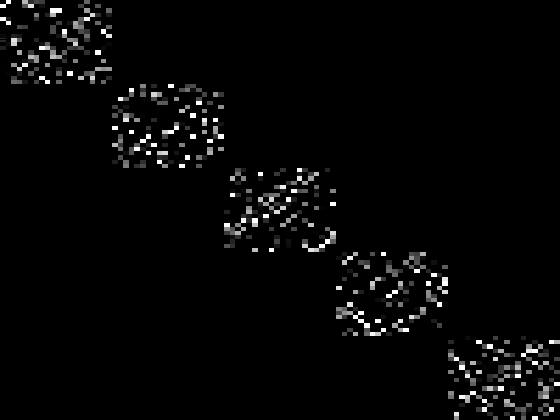
\includegraphics[width=0.35\linewidth]{pics/SEP.png}
  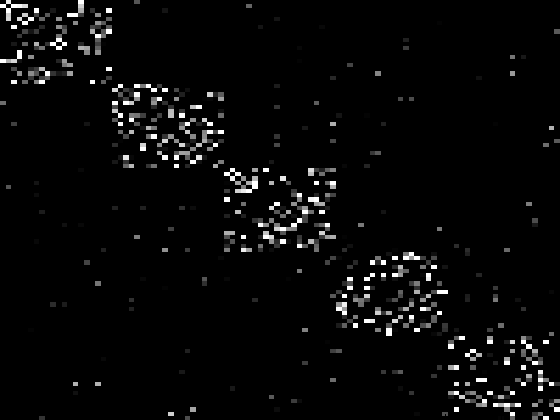
\includegraphics[width=0.35\linewidth]{pics/ViolateSEP.png}\\
  \caption{Illustration of LASSO-Subspace Detection Property/Self-Expressiveness Property. \textbf{Left:} SEP holds. \textbf{Right:} SEP is violated even though spectral clustering is likely to cluster this affinity graph perfectly into 5 blocks.}\label{fig:SEP}
\end{figure}

\paragraph{Models of analysis: }
Our objective here is to provide sufficient conditions upon which the LASSO subspace detection properties hold in the following four models. Precise definition of the noise models will be given in Section~\ref{sec:main}.

\begin{tabular}{ll}
  $\bullet$ fully deterministic model;\\
  $\bullet$ deterministic data with random noise;\\
  $\bullet$ semi-random data with random noise;\\
  $\bullet$ fully random model.
\end{tabular}




\section{主要结论}\label{sec:main}
\subsection{初步聚类的正确性}

\subsection{确定性模型}
%We start by defining some key concepts.
We start by defining two concepts adapted from the original proposal of \cite{soltanolkotabi2011geometric}.
\begin{definition}[投影对偶空间]\label{def:proj_dual_direction}
  令 $N$ 为下面对偶问题的最优解
  \begin{align*}
    \max_{N} \; \langle Y, N \rangle - \frac{1}{2\lambda}\| N
    \|_F^2,\quad\text{subject to:}\quad &\|N^T X\|_{2, \infty} \leq 1;
  \end{align*}
  $\mathcal{S}$ 为一个低维子空间。令$ \tilde{N} := \mathbb{P}_{\mathcal{S}} N$,
  对$\tilde{N}$ 进行紧致svd,有
  $$ \tilde{N} = \tilde{U} \Sigma V^T, \quad \tilde{U} \in \mathbb{R}^{d \times r}. $$
  则{\em 投影对偶空间} $\mathcal{U}$ 定义为
  $$\mathcal{U}(Y,X,\mathcal{S},\lambda)\triangleq \spa \{ \tilde{U}_i, i = 1\dots r \}.$$
\end{definition}
 %One way to interpret the optimal solution $N$ is that this is the Euclidean projection of $\lambda x$ to the polytope $\|X^TN\|_{\infty} \leq 1$ and $v$ is the direction of the projection of $N$ to subspace $\cS$.


\begin{definition}[投影子空间的非相干性]\label{def:incoherence}
  对于第$l$个子空间,我们指标集$I$,和其对应的投影对偶空间
  $\mathcal{U}_I^{(\ell)}=\mathcal{U}(X_I^{(\ell)},X_{I^c}^{(\ell)},\mathcal{S}_{\ell},\lambda)$。
  我们称集合 $\mathcal{X}_{\ell}$ 和其他点的不相干度为 $\mu$,如果
  \begin{align*}
    \mu\geq \mu(\mathcal{X}_{\ell}) := &\max_{y\in \mathcal{Y}\setminus \mathcal{Y}_{\ell}}
    \max_{I \in \mathcal{I}(l)} \|\mathbb{P}_{\mathcal{U_I}} y\|_2.
  \end{align*}
\end{definition}
%
%\begin{definition}[Incoherence property]
%There exists small constant $\mu$ such that
%\begin{align*}
%    \mu(S_{\ell}) := &\max_{y\in \mathcal{Y}\setminus \mathcal{Y}_{\ell}}{|\mathbb{P}_{S_{\ell}}(y)|}
%\end{align*}
%where $\mathbb{P}_{S_{\ell}}$ is the projection to subspace $S_{\ell}$.
%\end{definition}

Here, $\mu$ measures the incoherence between corrupted subspace samples $\mathcal{X}_{\ell}$ and clean data points in other subspaces (illustrated in Figure~\ref{fig:SubspaceIncoherence}). As $\|y\|=1$ by the normalization assumption, the range of $\mu$ is $[0,1]$. In case of random subspaces in high dimension, $\mu$ is close to zero. Moreover, as we will see later, for deterministic subspaces and random data points, $\mu$ is proportional to their expected angular distance (measured by cosine of canonical angles).

Definition~\ref{def:proj_dual_direction}~and~\ref{def:incoherence} differ from the \emph{dual direction} and \emph{subspace incoherence property} of \cite{soltanolkotabi2011geometric} in that we require a projection to a particular subspace to cater to the analysis of the noise case. Also, since they reduce to the original definitions when data are noiseless and $\lambda\rightarrow \infty$, these definitions can be considered as a generalization of their original version.

%\begin{figure}
%  \centering
%  % Requires \usepackage{graphicx}
%
%\end{figure}
\begin{figure}
  \centering
  % Requires \usepackage{graphicx}
  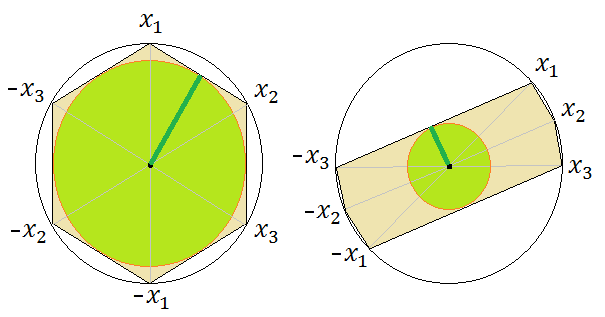
\includegraphics[width=0.7\linewidth]{pics/inradius.png}\\
  \caption{Illustration of inradius and data distribution. The inradius measures how well data points represent a subspace. }\label{fig:inradius}
  \includegraphics[width=0.9\linewidth]{pics/DualDirection.png}\\
  \includegraphics[width=0.9\linewidth]{pics/SubspaceIncoherence.png}
  \caption{Illustrations of the projected dual direction and subspace incoherence property. Jointly, $\left\{x \middle| \max_{i}\big|\langle v_i^{(\ell)},x\rangle\big|\leq \mu\right\}$ defines a polygon in the subspace $\cS_\ell$, and subspace incoherence $\mu$ is given by the smallest such polytope that contains the projections of all external point $y$ into the this subspace.}\label{fig:SubspaceIncoherence}
\end{figure}


%Compare to \citeauthor{soltanolkotabi2011geometric}'s original definition of dual direction and subspace incoherence, we add the projection to a particular subspace, which opens up the possibility for analysis under noise.

\begin{definition}[inradius]
The inradius of a convex body $\mathcal{P}$, denoted by $r(\mathcal{P})$, is defined as the radius of the largest Euclidean ball inscribed in $\mathcal{P}$.
\end{definition}
The inradius of a $\mathcal{Q}_{I^c}^{(\ell)}$ describes the dispersion of the data points. Well-dispersed data lead to larger inradius and skewed/concentrated distribution of data have small inradius. An illustration is given in Figure~\ref{fig:inradius}.


\begin{definition}[Deterministic noise model]
Consider arbitrary additive noise $Z$ to $Y$, each column $z_i$ is bounded by the two quantities below:
\begin{align*}
  \delta:= \max_i\|z_i\|, && \delta_1:=\max_{i,\ell}\|\mathbb{P}_\mathcal{S_{\ell}}z_i\|,
   %&& \delta_2:=\max_{i,\ell}\|\mathbb{P}_\mathcal{S_{\ell}^{\perp}}z_i\|.
\end{align*}
\end{definition}
As we assume the uncorrupted data point $y$ has unit norm, $\delta$ essentially describes the amount of allowable relative error.


\begin{theorem}\label{thm:thm_general}
Under the deterministic noise model, compactly denote
\begin{align*}
\mu_{\ell}:=\mu(\mathcal{X}_{\ell}),&& r_{\ell}:=\min_{\{i: x_i\in \mathcal{X}_{\ell}\}}r(\mathcal{Q}^{(\ell)}_{I^c}),&&
   r:=\min_{\ell=1,...,L} r_{\ell}.
\end{align*}
If $\mu_{\ell}< r_{\ell}$ for each $\ell = 1,...,L$, furthermore
$$ \delta\leq \min_{\ell=1,...,L}\frac{r(r_{\ell}-\mu_{\ell})}{2+7r_{\ell}} $$
then LASSO subspace detection property holds for all weighting parameter $\lambda$ in the range
\begin{equation*}
\frac{1}{r - 2\delta-\delta^2}<
        \lambda<\min_{\ell=1,..,L}\left\{\frac{r_{\ell}-\mu_{\ell}-2\delta_1}{\delta(1+\delta)(2+r_{\ell}-\delta_1)}\right\}
\end{equation*}
%\begin{equation*}
%\left\{\begin{aligned}
%  \lambda&>\frac{1}{(r-\delta_1)(1-3\delta) - 3\delta-2\delta^2}\\
%  \lambda&<\min_{\ell=1,..,L}\left\{\frac{r_{\ell}-\mu_{\ell}-2\delta_1}{\delta(1+\delta)(3+2r_{\ell}-2\delta_1)}\right\}\vee\frac{2r}{\delta^2(r+1)}.
%\end{aligned}\right.
%\end{equation*}
which is guaranteed to be non-empty.
\end{theorem}
We now offer some discussions of the theorem and the proof will be given in  Section~\ref{sec:proof_deterministic}.
%\begin{theorem}\label{thm:thm_general}
%Under deterministic noise model, compactly denote
%\begin{align*}
%  \rho:=2\lambda\delta(1+\delta),&&r:=\min_{\ell=1,...,k} \min_{\{i: x_i\in \mathcal{X}_{\ell}\}}r(\mathcal{Q}^{(\ell)}_{I^c}),&&\mu=\max_{\ell=1,...,k} \mu(\mathcal{X}_{\ell}).
%\end{align*}
%If $\mu< r$, furthermore
%$$ \delta\leq\frac{r(r-\mu)}{3r^2+7r+2}, $$
%then for each $\ell=1,...,k$, the solution $(c_i,e_i)$ to \eqref{eq:Opt_original} for $x_i\in \mathcal{X}_{\ell}$ satisfies:
%(1)$c_i \neq 0$,
%(2)support of $c_i$ corresponds to only columns of $X$ belonging to $\mathcal{X}_{\ell}$,
%for any weighting parameter $\lambda$ in the non-empty range:
%$$
%  \frac{1}{(r-\delta_1)(1-3\delta) - 2\delta}< \lambda < \min\left\{\frac{r-\mu-2\delta_1}{2\delta(1+\delta)(r-\delta_1+1)},\frac{2r}{\delta^2(r+1)}\right\}.
%$$
%\end{theorem}



%\begin{remark}[Noiseless case]
\paragraph{Noiseless case.} When $\delta=0$,  i.e., there is no noise, the condition reduces to $\mu_{\ell}< r_{\ell}$, which coincides with the result in \cite{soltanolkotabi2011geometric}. The exact LP formulation~\eqref{eq:SSC} is equivalent to $\lambda \rightarrow \infty$. Our result implies that unconstrained LASSO formulation \eqref{eq:Lasso} works for any $\lambda>\frac{1}{r}$. %{\color{red}[The last sentence is broken.]}
%\end{remark}

%\begin{remark}[Signal-to-Noise Ratio]
\paragraph{Signal-to-Noise Ratio.} Condition $\delta\leq\frac{r(r-\mu)}{2+7r}$ can be interpreted as the breaking point under increasing magnitude of attack. This suggests that SSC by \eqref{eq:Lasso} is provably robust to arbitrary noise having signal-to-noise ratio~(SNR) greater than $\Theta\big(\frac{1}{r(r-\mu)}\big)$. (Notice that $0<r<1$, and hence $7r+2 =\Theta(1)$.)
%\end{remark}

\paragraph{Tuning parameter $\lambda$.} The range of the parameter $\lambda$ in the theorem depends on unknown parameters $\mu$, $r$ and $\delta$, and therefore cannot be used in practice to choose the parameter in practice. It does however justify that when $\delta$ is small, the range of $\lambda$ that Lasso-SSC works is large, therefore not hard to tune. In practice, we do not need to know $\lambda$ in prior. One approach is to trace the Lasso path \cite{tibshirani2013lasso} until we have about $k$ non-zero entries in the coefficient vector. If we would like to use a single $\lambda$ for all columns, a good point to start is to take $\lambda$ to be in the order of $O\big(\frac{1}{\min_j \max_{i\neq j}|x_i^Tx_j|}\big)$, this ensures the solution to be at least non-trivial.


\paragraph{Agnostic subspace clustering.}
The robustness to deterministic error is important, since in practice the union-of-subspace structures are usually only good approximations. If each subspace has decaying singular values (e.g., motion segmentation, face clustering \cite{elhamifar2012ssc_journal} and hybrid system identification\cite{vidal2003algebraic}), the deterministic guarantee allows for the flexibility in choosing the cut-off points, e.g., take 90\% of the energy as signal and treat the remaining spectrum as noise. If one keeps a smaller number of singular values ( a smaller subspace dimension), the inradius will likely to be larger \footnote{A formal relationship between inradius and smallest singular value is described in \cite{wang2013provable}.}, although the noise level also increases. It is  possible that the conditions in Theorem~\ref{thm:thm_general} are satisfied for some decomposition (e.g., those with a large spectral gap) but not others. The nice thing is that this is not a tuning parameter, but rather a theoretical property that remains agnostic to the users. In fact, the algorithm will be provably effective as long as the conditions are satisfied for any signal noise decomposition (not restricted to rank-projection). None of these is possible if distributional assumptions are made to either the data or the noise.








%\begin{figure}
%  \centering
%  \includegraphics[width=0.8\textwidth]{pics/Noiseless_vs_Noisy.png}\\
%   \caption{Geometric interpretation and comparison of the noiseless SSC (\textbf{Left}) and noisy LASSO-SSC (\textbf{Right}).}
%   \label{fig:geom_interpretation}
%\end{figure}



%\begin{figure}
%  \centering
%  \includegraphics[width=7cm]{pics/NoiselessGuarantee.png}\\
%   \caption{Noiseless SSC: Theorem~2.5 of \cite{soltanolkotabi2011geometric} suggests that the projection of external data points must fall inside the solid blue polygon, which is the intersection of halfspaces defined by dual directions (blue dots) that are tangent planes of the red inscribing sphere.}
%   \label{fig.noiseless_guarantee}
%\end{figure}
%\begin{figure}
%  \centering
%  \includegraphics[width=7cm]{pics/NoisyGuarantee.png}\\
%  \caption{Noisy LASSO-SSC: The guarantee of Theorem~\ref{thm:thm_general} means that the whole red sphere of each external data points must fall inside the dashed red polygon, which is smaller than the blue polygon by a factor related to the noise level. } \label{fig.noisy_guarantee}
%\end{figure}

\subsection{Randomized models}
We  further analyze three randomized models with increasing level of randomness.
\begin{description}
  \item[$\bullet$ Determinitic+Random Noise.] Subspaces and samples in subspace are arbitrary; the noise obeys the Random Noise model (Definition~\ref{def:Random_noise_model}).
  \item[$\bullet$ Semi-random+Random Noise.] Subspace is deterministic, but samples in each subspace are drawn iid uniformly from the intersection of the unit sphere and the subspace; the noise obeys the Random Noise model.
  \item[$\bullet$ Fully random.] Both subspace and samples are drawn uniformly at random from their respective domains; the noise is iid Gaussian.%\footnote{It is straightforward to state the model for Definition~\ref{def:Random_noise_model}. We choose Gaussian as an illustration.}.
\end{description}

\begin{definition}[Random noise model]\label{def:Random_noise_model}
Our random noise model is defined to be any additive $Z$ that is (1) columnwise iid; (2) spherical symmetric;  and (3) $\|z_i\|\leq \delta$ for all $i=1,...,N$ with probability at least $1-1/N$.
\end{definition}
%\begin{example}[Gaussian noise]
$$\P\left(\delta:=\max_i\|z_i\| > \sqrt{1+\frac{6\log N}{n}}\sigma\right) \leq C/N^2.$$
%\end{example}

\begin{theorem}[Deterministic+Random Noise]\label{thm:thm_random_noise}
 Under random noise model, compactly denote $r_{\ell}$, $r$ and $\mu_{\ell}$ as in Theorem~\ref{thm:thm_general}, furthermore let
$$\epsilon := \sqrt{\frac{6\log N}{n-\max_{\ell}{d_{\ell}}}}\leq \sqrt{\frac{C\log(N)}{n}}.$$
 %$$\epsilon := \sqrt{\frac{6\log N+2\log \max_{\ell}{d_{\ell}}}{n-\max_{\ell}{d_{\ell}}}}\leq \sqrt{\frac{C\log(N)}{n}} .$$
 If $\mu_{\ell}<r_{\ell}$ for all $\ell = 1,...,k$,
 \begin{align*}
 \epsilon\delta<\min_{\ell=1,...,L}\frac{r_{\ell}-\mu_{\ell}}{2\sqrt{d_{\ell}}+2}, &&\text{and}&& \epsilon\delta(1+\delta) < \min_{\ell=1,...,L}\frac{r(r_\ell-\mu_\ell)}{4r_\ell+6},
\end{align*}
 %$$\delta<\min_{\ell=1,...,L}\frac{r_{\ell}-\mu_{\ell}}{2r_{\ell}+4},$$
then with probability at least $1-9/N$, LASSO subspace detection property holds for all weighting parameter $\lambda$ in the range
\begin{equation}\label{eq:thm_rand_noise_lambda_range}
\frac{1}{r- 2\epsilon \delta-\epsilon\delta^2}<
        \lambda<\min_{\ell=1,...,L}\left\{\frac{r_{\ell}-\mu_{\ell}-\delta\epsilon - \delta \sqrt{d_{\ell}} \epsilon}{\epsilon\delta(1+\delta)(3+r_{\ell}-\delta\sqrt{d_{\ell}}\epsilon)}\right\}
%\frac{1}{(r-\delta\epsilon)(1-2\delta) - 2\delta-\delta^2}<
%        \lambda<\min_{\ell=1,...,L}\left\{\frac{r_{\ell}-\mu_{\ell}-2\delta\epsilon}{\epsilon\delta(1+\delta)(2+r_{\ell}-\delta\epsilon)}\right\}
\end{equation}
which is guaranteed to be non-empty.
\end{theorem}
\paragraph{Low SnR paradigm.} Compared to Theorem~\ref{thm:thm_general}, Theorem~\ref{thm:thm_random_noise} considers a more benign noise which leads to a stronger result. In particular, without assuming any statistical model on how data are generated, we show that Lasso-SSC is able to tolerate noise of level $O\left((\frac{n}{\log N})^{1/4}(r(r_\ell-\mu_\ell))^{1/2}\right)$ or $O\left((\frac{n}{d\log N})^{1/2}(r_\ell-\mu_\ell)\right)$ (whichever is smaller). This extends SSC's guarantee with deterministic data to cases where the noise can be significantly larger than the signal. In fact, the SnR can go to $0$ as the ambient dimension gets large.

On the other hand, Theorem~\ref{thm:thm_random_noise} shows that Lasso-SSC is able to tolerate a constant level of noise when the geometric gap $r_\ell-\mu_\ell$ is as small as $O(\sqrt{d/n})$. This is arguably near-optimal (when $d$ is small) as the projection of a constant-level random noise into a $d$-dimensional subspace has an expected magnitude of the same order, which could easily close up the small geometric gap for some non-trivial probability if the noise is much larger.

%We note that the projection of the random noise into the subspace ($\delta_1$) has the magnitude of the same order $O(\sqrt{d/n})$. {\color{red}[Not sure what the last sentence means.]} % I was intending to argue that this is big enough to distort everything in the subspace almost arbitrarily.


\paragraph{Margin of error.}
Since the bound depends critically on $(r_\ell-\mu_\ell)$~--~the difference of inradius and incoherence~--~which is the geometric gap that appears in the noiseless guarantee of \cite{soltanolkotabi2011geometric}. We will henceforth call this gap the \emph{margin of error}.

We now analyze this margin of error under different generative models. We
start from the semi-random model, where the distance between two subspaces is measured as follows.
\begin{definition}\label{def:subspace_affinity}
The {\em affinity} between two subspaces is defined by:
$$ \mathrm{aff}(\mathcal{S}_k,\mathcal{S}_{\ell}) = \sqrt{\cos^2{\theta^{(1)}_{k\ell }}+...+\cos^2{\theta^{(\min(d_k,d_{\ell}))}_{k\ell}}},$$
where $\theta_{k\ell}^{(i)}$ is the $i^{th}$ canonical angle between the two subspaces. Let $U_{k}$ and $U_{\ell}$ be a set of orthonormal bases of each subspace, then $\mathrm{aff}(\mathcal{S}_k,\mathcal{S}_{\ell})=\|U_{k}^TU_{\ell}\|_F$.
\end{definition}
When data points are randomly sampled from each subspace, the geometric entity $\mu(\mathcal{X}_{\ell})$ can be expressed using this (more intuitive) subspace affinity, which leads to the following theorem.


\begin{theorem}[Semi-random model+random noise]\label{thm:semirandom}
Under the semi-random model with random noise, there exists a non-empty range of $\lambda$ such that LASSO subspace detection property holds with probability $1- \frac{9}{N} - \frac{1}{L^2}\sum_{\ell\neq \ell^\prime}\frac{1}{(N_{\ell}+1)N_{\ell^\prime}} e^{-\frac{t}{4}} -6\sum_{\ell=1}^L (e^{\gamma_1 (n-d_\ell)}+e^{\gamma_2 d_\ell}+e^{-\sqrt{N_{\ell}d_{\ell}}})$ as long as the noise level obeys
\begin{align*}
 \delta(1+\delta) \leq& \max_{\ell,\ell'}\sqrt{\frac{n-d}{6\log N}} \frac{\sqrt{\log \kappa}}{40K_2\sqrt{dd_\ell}}\left(1- \frac{K_1K_2 \mathrm{aff}(\mathcal{S}_{\ell},\mathcal{S}_{\ell^\prime})}{\sqrt{ d_{\ell^\prime}}} \right),
\end{align*}
where $K_1:= (t \log  [(N_{\ell}+1)N_{\ell^\prime}] + \log L)$, $K_2 := 4\sqrt{\frac{1}{\log\kappa_\ell}}$, $\kappa_\ell := N_{\ell}/d_{\ell}$, $\frac{\log\kappa}{d} :=\min_{\ell} \frac{\log\kappa_\ell}{d_\ell}$, and
$\gamma_1,\gamma_2$ are absolute constants.
\end{theorem}
The proof is essentially substituting the incoherence and inradius parameters in Theorem~\ref{thm:thm_random_noise} with meaningful bounds, so Thereom~\ref{thm:semirandom} can be regarded as a corollary of Theorem~\ref{thm:thm_random_noise}.

\paragraph{Overlapping subspaces.}
Similar to the results in \cite{soltanolkotabi2011geometric}, Theorem~\ref{thm:semirandom} demonstrates that LASSO-SSC can handle overlapping subspaces with noisy samples. By Definition~\ref{def:subspace_affinity}, $\mathrm{aff}(\mathcal{S}_k,\mathcal{S}_{\ell})$ can be small even if $\mathcal{S}_k$ and $\mathcal{S}_{\ell}$ share a basis.

\paragraph{Comparison to \cite{soltanolkotabi2013robust}.}
In the high dimensional setting when $n\gg d$, our result is able to handle the low SnR regime when $\delta = \Theta(n^{1/4}/d^{1/2})$, while \cite{soltanolkotabi2013robust} needs $\delta$ to be bounded by a small constant.

In the case when $d$ is a constant fraction of $n$, however, our bound is worse by a factor of $\sqrt{d}$. \cite{soltanolkotabi2013robust} is still able to handle a small constant noise while we needs $\delta < O(\frac{1}{\sqrt{d}})$. The suboptimal bound might be due to the fact that we are simply developing the theorem for the semirandom model as a corollary of Theorem~\ref{thm:thm_random_noise} and haven not fully exploit the structure of the semi-random model in the proof.

%Lastly, our result does not invoke the Restricted Isometry Property (RIP) bound at any point of the analysis therefore does not have any restrictions on the subspace dimension.  %The point is made more explicitly in the fully random model in Theorem~\ref{thm:fullrandom2}.
%In fact, if we are willing to assume $d>\log N$, we can apply the intermediate results in the proof of \cite{soltanolkotabi2013robust} to further improve the bound to handle $\delta = \Theta((n/d)^{1/4})$ (see appendix for details), this matches the best known results for noisy subspace clustering using TSC \cite{heckel2013robust}.


We now turn to the fully random case.
\begin{theorem}[Fully random model]\label{thm:fullrandom}
Suppose there are $L$ subspaces each with dimension $d$, chosen independently and uniformly at random. For each subspace, $\kappa d+1$ points are chosen independently and uniformly from the unit sphere inside each subspace. Each measurement is corrupted by iid Gaussian noise $\sim N(0,\sigma^2/n)$. Furthermore, if
\begin{align*}
  d < \frac{c(\kappa)^2\log\kappa}{24\log N} n, &&\text{and} && \sigma(1+\sigma) < \frac{c(\kappa)^2\log \kappa  }{20}\frac{\sqrt{n} }{d},
\end{align*}
then with probability at least $1-\frac{10}{N}-Ne^{-\sqrt{\kappa}d}$, the LASSO subspace detection property holds for any $\lambda$ in the range
\begin{equation}\label{eq:thm_rand_lambda_range}
  \frac{C_1\sqrt{d}}{c(\kappa)\sqrt{\log \kappa}}<\lambda <  \frac{C_2c(\kappa)\sqrt{n\log\kappa}}{\sigma\sqrt{d\log N}},
\end{equation}
which is guaranteed to be non-empty. Here, $C_1,C_2$ are absolute constants.
\end{theorem}
The results under this simple model are very interpretable. It
 provides intuitive guideline in how robustness of Lasso-SSC change with respect to the various parameters of the data.
 One one hand, it is sensitive to the dimension of each subspace $d$, since the $\sigma \leq \tilde{\Theta}(\frac{n^{1/4}}{\sqrt{d}})$. This dependence on subspace dimension $d$ is not a critical limitation as most interesting applications indeed have very low subspace-dimension, as summarized in Table~\ref{tab:low_rank}.
On the other hand, the dependence on the number of subspaces $L$ (in both $\log\kappa$ and $\log N$ since $N=L(\kappa d+1)$) is only logarithmic.  This suggests that SSC is robust even when there are many clusters, and $Ld\gg n$.

% such as subspace dimension $d$ and number of subspaces $L$ in the simplistic setting.



%
%\begin{remark}[Trade-off between $d$ and the margin of error]\label{rmk:tradeoff_large_d}
%Theorem~\ref{thm:fullrandom}  extends our results to the paradigm where the subspace dimension grows  linearly with the ambient dimension. Interestingly, it shows that the margin of error scales $\tilde{\Theta}(\sqrt{1/d})$, implying a relationship between $d$ and robustness to noise. Fortunately,  most interesting applications indeed have very low subspace-rank, as summarized in Table~\ref{tab:low_rank}.
%\end{remark}



\begin{table}
  \centering
 \begin{tabular}{|p{0.6\linewidth}|c|}
   \hline
   % after \\: \hline or \cline{col1-col2} \cline{col3-col4} ...
   \textbf{Application} & \textbf{Cluster rank}\\
   \hline
   3D motion segmentation \cite{costeira1998motion_seg} & $\mathrm{rank}=4$ \\\hline
   Face clustering (with shadow) \cite{basri2003lambertianface} & $\mathrm{rank}=9$ \\\hline
   Diffuse photometric face \cite{zhou2007PhotometricFace}& $\mathrm{rank}=3$ \\\hline
   Network topology discovery \cite{eriksson2011high_rankMC} & $\mathrm{rank}=2$ \\\hline
   Hand writing digits \cite{hastie1998MNIST}&  $\mathrm{rank}=12$\\\hline
   Social graph clustering \cite{xu2011graphclustering}& $\mathrm{rank}=1$ \\
   \hline
 \end{tabular}
  \caption{Rank of real subspace clustering problems}\label{tab:low_rank}
\end{table}

%\begin{remark}[Robustness in the many-cluster setting]\label{rmk:large_num_subspace}
%Another interesting observation is that the margin of error scales logarithmically with respect to $L$, the number of clusters (in both $\log\kappa$ and $\log N$ since $N=L(\kappa d+1)$). This suggests that SSC is robust even if there are many clusters, and $Ld\gg n$.
%\end{remark}



%\noindent\textbf{The guarantee in Theorem~\ref{thm:thm_general}:}
\subsection{Geometric interpretations}%  of Theorem~\ref{thm:thm_general}}
A geometric illustration of the condition in Theorem~\ref{thm:thm_general} is given in Figure~\ref{fig:geom_interpretation} in comparison to the geometric separation condition in the noiseless case.

\begin{figure}
        \centering
        \begin{subfigure}[t]{0.4\textwidth}
          \centering
              \includegraphics[width=\textwidth]{pics/NoiselessGuarantee.png}\\
               \caption{Noiseless SSC}
               \label{fig.noiseless_guarantee}
        \end{subfigure}%
        ~ %add desired spacing between images, e. g. ~, \quad, \qquad etc.
          %(or a blank line to force the subfigure onto a new line)
        \begin{subfigure}[t]{0.4\textwidth}
              \centering
              \includegraphics[width=\textwidth]{pics/NoisyGuarantee.png}\\
              \caption{Noisy LASSO-SSC} \label{fig.noisy_guarantee}
        \end{subfigure}
   \caption{Geometric interpretation and comparison of the noiseless SSC (\textbf{Left}) and noisy LASSO-SSC (\textbf{Right}).
   %On the \textbf{left}, Theorem~2.5 of \cite{soltanolkotabi2011geometric} suggests that the projection of external data points must fall inside the solid blue polygon, which is the intersection of halfspaces defined by dual directions (blue dots) that are tangent planes of the red inscribing sphere. On the \textbf{right}, the guarantee of Theorem~\ref{thm:thm_general} means that the whole red sphere of each external data points must fall inside the dashed red polygon, which is smaller than the blue polygon by a factor related to the noise level.
   }
   \label{fig:geom_interpretation}
\end{figure}

The left pane depicts the separation condition $\mu_\ell \leq r_\ell$ in Theorem~2.5 of \cite{soltanolkotabi2011geometric}. The blue polygon represents the the intersection of halfspaces defined with dual directions that are also the tangent to the red inscribing sphere. More precisely, this is $\left\{x\in \cS_\ell \middle| \big|\langle v_i^{\ell}, x\rangle\big| \leq r_\ell\right\}$. From our illustration of $\mu$ in Figure~\ref{fig:SubspaceIncoherence}, we can easily tell that $\mu_\ell\leq r_\ell$ if and only if the projection of external data points fall inside this solid blue polygon. We call this solid blue polygon the successful region.

The right pane illustrates our guarantee of Theorem~\ref{thm:thm_general} under bounded deterministic noise. The successful condition requires that the whole red ball (analogous to uncertainty set in Robust Optimization \cite{ben1998robust,bertsimas2004price}) around each external data point to fall inside the dashed red polygon, which is smaller than the blue polygon by a factor related to the noise level and the inradius.

The successful region is affected by the noise because the design matrix is also arbitrarily perturbed and the dual solution is no longer within each subspace $\cS_\ell$. Specifically, as will become clear in the proof, the key of showing SEP boils down to proving
$
\langle N_i^{(\ell)}, x_j\rangle < 1
$
for all pairs of $(N_i^{(\ell)}, x_j)$ where
$$ N_i^{(\ell)}=\arg\max_{N} \langle N, x_i^{(\ell)}\rangle  -\frac{1}{2\lambda}\|N\|^2 \text{ s.t. }  \|N^TX_{I^c}^{(\ell)} \|_\infty \leq 1,$$
and $x_j$ is any point from another subspace. In the noiseless case we can always take $N_i^{(\ell)}\in\cS_\ell$ and $\langle N_i^{(\ell)}, x_j\rangle \leq \frac{\mu_\ell}{r_\ell}$. For noisy data and Lasso-SSC, we can no longer do that. In fact, for any fixed $\lambda$, the dual solution will be uniquely determined by a projection of $\lambda x_i^{(\ell)}$ on to the feasible region $\|N^TX_{I^c}^{(\ell)} \|_\infty \leq 1$ (see the first pane of Figure~\ref{fig:SubspaceIncoherence}). The absolute value of the inner product $\langle N_i^{(\ell)}, x_j\rangle$ will depend on the magnitude of the dual solution, especially its component perpendicular to the current subspace. Indeed by carefully choosing the error, we can make $\mathbb{P}_{\cS_\ell^{\perp}}N$ very correlated with some external data point $x_j$.

%This is why we need to shrink the size of the successful region to account for the worst case.

To illustrate this further, we plot the shape of this feasible region in 3D (see Figure~\ref{fig.convex_hull_n_polar}(b)). From the feasible region alone, it seems that the magnitude of dual variable can potentially be quite large. Luckily, the quadratic penalty in the objective function allows us to exploit the optimality of the solution $N$ and bound the ``out-of-subspace'' component of $N$, which results in a much smaller region where the solution can potentially be (given in Figure~\ref{fig.convex_hull_n_polar}(c)). The region for the ``in-subspace'' component is also smaller as is shown in Figure~\ref{fig.ProjPolar}. A more detailed argument of this is given in Section~\ref{sec:dual_separation} of the proof.

\begin{figure}
  \centering
%  % Requires \usepackage{graphicx}
%  \includegraphics[width=0.6\linewidth]{pics/CandesDualDirection.png}\\
%  \caption{An illustration of dual direction from \cite{soltanolkotabi2011geometric}.}\label{fig.candes_dual_direction}
    \includegraphics[width=0.7\linewidth]{pics/conv_hull_n_polarset2.png}\\
  \caption{Illustration of \textbf{(a)} the convex hull of noisy data points, \textbf{(b)} its polar set and \textbf{(c)} the intersection of polar set and $\|N_{\parallel}\|$ bound. The polar set (b) defines the feasible region of \eqref{eq:dual_fictitious2}. It is clear that $N_{\parallel}$ can take very large value in (b) if we only consider feasibility. By considering optimality, we know the optimal $N$ must be inside the region in (c).} \label{fig.convex_hull_n_polar}
    \includegraphics[width=0.6\linewidth]{pics/Projected_polarset_cmp1.png}\\
  \caption{The projection of the polar set (the green area) in comparison to the projection of the polar set with $\|N_{\parallel}\|$ bound (the blue polygon). It is clear that the latter is much smaller.}\label{fig.ProjPolar}
\end{figure}

Admittedly, the geometric interpretation under noise is slightly messier than the noiseless case, but it is clear that the largest deterministic noise Lasso-SSC can tolerate must be smaller than geometric gap $r_\ell-\mu_\ell$. Theorem~\ref{thm:thm_general} show that a sufficient condition is $\delta \leq O(r(r_\ell-\mu_\ell))$. It remains unclear whether this gap can be closed without additional assumptions.

%\subsection{Geometric interpretation of Theorem~\ref{thm:thm_random_noise}}

Finally, we note that for the random noise model in Theorem~\ref{thm:thm_random_noise}, the geometric interpretation is similar, except that the impact of the noise is weakened. Thanks to the randomness and the corresponding concentration of measure, we may bound the reduction of the successful region with a much smaller value comparing to the adversarial noise case.

%Algebraically, this is made clear by the \emph{randomized dual separation condition} (see \eqref{eq:dual_sep_random} in Lemma~\ref{lemma:dual_sep_random}). From the robust optimization perspective, this is equivalent to reducing the size of the uncertainty set by leaving the bulk unlikely region of the uncertainty set unconstrained. In other word, the size of the red ball in Figure~\ref{fig:geom_interpretation} is much smaller in the randomized case.







\section{初步聚类的正确性}\label{sec:proof_greedy}
下面是 Levy 引理的特殊形式。
\begin{lemma}[\cite{ledoux2005concentration}] \label{lem:measureconc}
对 $x \sim \text{Unif}(\mathbb{S}^{d-1})$,我们有
\begin{align*} 
\Pr \{ \| A x \|_2  > m\|A x\|_2 + t \} &\le \exp \left( - \frac{dt^2}{2\|A\|_2^2} \right), \\
\Pr \{ \| A x \|_2  < m\|A x\|_2 - t \} &\le \exp \left( - \frac{dt^2}{2\|A\|_2^2} \right).
\end{align*}
对任意 $A \in \R^{p \times d}, t > 0$ 成立。 其中$m\|Ax\|_2$ 是 $\|Ax\|_2$ 的中位数。
\end{lemma}

\begin{lemma} \label{lem:expectation}
  对 $x \sim \text{Unif}(\mathbb{S}^{d-1})$ 和任意矩阵 
  $A \in \mathbb{R}^{p \times d}$,我们有
  $$ E[\|Ax\|_2^2] = \frac{1}{d} \|A\|_F^2 $$
\end{lemma}

\begin{proof}
令 $A = U \Sigma V^T$ 为 $A$ 的奇异值分解,于是
\begin{align*}
  E[\|Ax\|_2^2] = E[\|U \Sigma V^T x\|_2^2] 
  = E[\|\Sigma x\|_2^2] = \sum_{i=1}^{\min(p,d)} \sigma_i^2 E[x_i^2] 
  = \sum_{i=1}^{\min(p,d)} \sigma_i^2 \cdot \frac{1}{d} = \frac{1}{d} \|A\|_F^2.
\end{align*}
其中$ E[x_i^2] = \frac{1}{d}$,是因为 $x$ 的每个分量对称,期望相同,而$ \sum_{i=1}^d E[x_i^2] = 1 $,
\end{proof}

\begin{lemma} \label{lem:subspace_concentration}
  对 $x \sim \text{Unif}(\mathbb{S}^{d-1})$ 和任意矩阵 
  $A \in \mathbb{R}^{p \times d}$,若 $\|A\|_2$ 有界,我们有
  \begin{align*}
    \Pr \left\{ \|A x\|_2 > \sqrt{\frac{1}{d}} \|A\|_F + 
    \|A\|_2 \cdot \left( \sqrt{\frac{2\pi}{d}} + \delta \right) \right\}
    \le e^{-\frac{d \delta^2}{2}},
  \end{align*}
  其中$\delta$ 为任意正实数。
\end{lemma}

\begin{proof}
  由引理\ref{lem:measureconc},我们有
  \begin{align*}
    \left| E\|A x\|_2 - m\|A x\|_2 \right| &\le E\left[ \left| \|A x\|_2 - m\|A x\|_2 \right| \right] \le \int_0^\infty 2e^{-\frac{dt^2}{2\|A\|_2^2}} dt = \sqrt{\frac{2\pi}{d}} \|A\|_2.
  \end{align*}
  于是
  \begin{align*}
    \Pr \left\{ \|A x\|_2 > \sqrt{\frac{\|A\|_F^2}{d}} + \sqrt{\frac{2\pi}{d}} \|A\|_2 + t \right\}
    &= \Pr \left\{ \|A x\|_2 > \sqrt{E\|A x\|_2^2} + \sqrt{\frac{2\pi}{d}} \|A\|_2 + t \right\} \\
    &\le \Pr \left\{ \|A x\|_2 > E\|A x\|_2 + \sqrt{\frac{2\pi}{d}} \|A\|_2 + t \right\} \\
    &\le \Pr \left\{ \|A x\|_2 > m\|A x\|_2 + t \right\} \\
    &\le \exp \left( -\frac{dt^2}{2 \|A\|_2^2} \right).
  \end{align*}
  其中由Jensen 不等式 $ E\|A x\|_2 \le \sqrt{E\|Ax\|_2^2}$,
  由引理\ref{lem:subspace_concentration} $E \|Ax\|_2^2=\frac{\|A\|_F^2}{d}$。
  另$\delta = \frac{t}{\|A\|_2}$ 即得证。
\end{proof}

为了控制当前点与
\begin{lemma}[\cite{ball1997intro_convex_geometry}]\label{lem:spherical_cap}
  对 $x \sim \text{Unif}(\S^{d-1})$ 和任意固定的向量 $a$,我们有
  \begin{align*}
    \left( \frac{1-\varepsilon}{2} \right)^{\frac{d-1}{2}} \ge
    \Pr\left(|a^Tx|>\epsilon \|a\|_2\right) \leq 2e^{\frac{-d\epsilon^2}{2}}
  \end{align*}
\end{lemma}

\begin{lemma} \label{lem:projbound_upper}
  设 $x_1, \ldots, x_n $ 为采样于$\text{Unif}(\S^{d-1})$ 的独立同分布随机向量,
  令 $z$ 为 $\{ |a^T x_i|, 1 \le i \le n\}$
  中的最大值,其中$a \in \R^d $ 是固定向量,则
  \begin{align*}
    \Pr{z>\sqrt{\frac{2}{d} \log \frac{2n}{\delta}} \|a\|_2} \le \delta,
  \end{align*}
  其中$0<\delta<1$。
\end{lemma}

\begin{proof}
  对任意$\varepsilon>0$,我们有
  \begin{align*}
    \Pr{z > \varepsilon \|a\|_2} &\le \Pr\left\{\exists i \in [n] : |a^T
    x_i|>\varepsilon \|a\|_2 \right\} \\
    &\le n \Pr\left\{ |a^T x_i|>\varepsilon \|a\|_2\right\} \\
    &\le 2n e^{\frac{-d\varepsilon^2}{2}},
  \end{align*}
  其中第三个不等式用了引理\ref{lem:spherical_cap}。令$\delta=2n
  e^{\frac{-d\varepsilon^2}{2}}$即得证。
\end{proof}

\begin{lemma} \label{lem:projbound_lower}
  设 $x_1, \ldots, x_n $ 为采样于$\text{Unif}(\S^{d-1})$ 的独立同分布随机向量,
  令 $z_m$ 为 $\{ |a^T x_i|, 1 \le i \le n\}$ 中的第m大值,其中$a \in \R^d $ 是固定向量,则
  \begin{align*}
    \Pr\left\{z_m>\left( 1-2\left(\frac{m\log \frac{ne}{m}-\log \delta}{n-m+1}
    \right)^{\frac{2}{d-1}}\right) \|a\|_2\right\} \ge 1-\delta,
  \end{align*}
  其中$0<\delta<1$。
\end{lemma}
\begin{proof}
  对任意$\varepsilon>0$,我们有
  \begin{align*}
    \Pr\{z_m \le \varepsilon \|a\|_2\} &= \Pr\left\{\exists I \subset [n], |I|=n-m+1:
    z_i \le \varepsilon, \forall i \in I\right\} \\
    &\le \binom{n}{m-1} \cdot \Pr \left\{ z_1 \le \varepsilon \right\}^{n-m+1}\\
    &\le \left( \frac{ne}{m} \right)^m \cdot \left( 1-\left(
    \frac{1-\varepsilon}{2} \right)^{\frac{d-1}{2}} \right)^{n-m+1} \\
    &\le \exp \left\{ m \log \frac{ne}{m}-\left(
    \frac{1-\varepsilon}{2}\right)^{\frac{d-1}{2}} (n+m-1) \right\},
  \end{align*}
  其中我们用了引理\ref{lem:spherical_cap}, $\binom{n}{m}\le
  (\frac{ne}{m})^m$ 和 $1+x\le e^x, \forall x$。
  令
  $$\delta= \exp \left\{ m \log \frac{ne}{m}-\left(
    \frac{1-\varepsilon}{2}\right)^{\frac{d-1}{2}} (n+m-1)
  \right\}$$
  再取互补事件即可得证。
\end{proof}

为了保证算法\ref{alg:nsn}的正确性,我们要求对每个点,它的$k$邻居点都和自身属于同一
子空间。不是一般性,我们这就意味着
$$ |x_1^T x_i|>|x_1^T x_j| \forall j \in {j:l_j \ne l_1 $$
\section{确定情形下的证明}\label{sec:proof_deterministic}

%,\ref{thm:thm_random_noise},\ref{thm:semirandom}~and~\ref{thm:fullrandom}.
我们不直接分析\eqref{eq:Lasso},而是引入松弛变量$E_I$,将其转化为有限制的等价形式:
\begin{align}\label{eq:Opt_original}
  \mathbf{P}_0:\quad \min_{C_I, E_I} \;
  \|C_I^T\|_{2,1}+\frac{\lambda}{2}\|E_I\|_F^2 \quad
  s.t. \quad X^{(\ell)}_I=X_{I^c}C_I+E_I.
\end{align}
The constraint can be rewritten as
\begin{equation}\label{eq:Opt_original_equi}
  y^{(\ell)}_i+z^{(\ell)}_i=(Y_{I^c}+Z_{I^c})c_i+e_i.
\end{equation}
The dual program of \eqref{eq:Opt_original} is:
\begin{equation}\label{eq:Opt_original_dual}
  \begin{aligned}
    \mathbf{D}_0:\quad \max_{N} \; \langle x_i,N \rangle - \frac{1}{2\lambda}N^TN \quad
    s.t. \quad \|(X_{I^c})^TN\|_{\infty} \leq 1.
  \end{aligned}
\end{equation}
Recall that we want to establish the conditions on noise magnitude $\delta$, structure of the data ($\mu$ and $r$ in the deterministic model and affinity in the semi-random model), and ranges of valid $\lambda$ such that by Definition~\ref{def:lasso_detection}, the solution $c_i$ is \emph{non-trivial} and has support indices inside the column set $X^{(\ell)}_{I^c}$ (i.e., satisfies SEP).
考虑一个一般的凸优化问题:
\begin{align}\label{eq:Opt_A_general}
  \quad \min_{C, E} \; &\|C^T\|_{2,1}+\frac{\lambda}{2}\|E\|^2_F \quad &s.t. \quad Y=XC+E.
\end{align}
We state Lemma~\ref{lemma:OptimalCondition}, which extends Lemma~7.1 in \cite{soltanolkotabi2011geometric}.
\begin{lemma}\label{lemma:OptimalCondition}
  考虑矩阵$X\in \mathbb{R}^{d\times n}$和矩阵$Y \in \mathbb{R}^{d\times n}$.
  如果存在三元组 $(C,E,N)$ 满足 $Y=XC+E$, $C$ 的行支撑集 $S\subseteq T$,$N$满足
  \begin{equation*}
    \begin{array}{cc}
      N^T X_S = \norm(C_S^T),  & N=\lambda E, \\
      \|N^T X_{T\cap S^{c}}\|_{2, \infty} \leq 1, & \|N^T X_{T^{c}}\|_{2, \infty}<1,
    \end{array}
  \end{equation*}
  则\eqref{eq:Opt_A_general} 的任意最优解 $(C^{*},E^{*})$ 必然有
  $(C^{*})^T_i=\mathbf{0} \quad \forall i \in T^c$.
\end{lemma}

\begin{proof}
  对最优解 $(C^{*},E^{*})$, 我们有:
  \begin{align}
    &\|(C^*)^T\|_{2,1}+\frac{\lambda}{2}\|E^*\|_F^2 \nonumber\\
    =& \|(C^*)^T_S\|_{2,1}+\|(C^*)^T_{T\cap
    S^c}\|_{2,1}+\|(C^*)^T_{T^c}\|_{2,1} + \frac{\lambda}{2} \|E^*\|^2_F\nonumber\\
    \geq&\|C^T_S\|_{2,1}+\langle \norm(C_S),C^*_S-C_S\rangle+\|(C^*)^T_{T\cap
    S^c}\|_{2,1}+\|(C^*)^T_{T^c}\|_{2,1} + \frac{\lambda}{2} \|E\|^2_F +\langle
    \lambda E,E^*-E\rangle\nonumber\\
    =&\|C^T_S\|_{2,1}+\langle N,X_S(C^*_S-C_S)\rangle+\|(C^*)^T_{T\cap
    S^c}\|_{2,1}+\|(C^*)^T_{T^c}\|_{2,1} + \frac{\lambda}{2} \|E\|^2_F +\langle
    \lambda E,E^*-E\rangle\nonumber\\
    =&\|C^T_S\|_{2,1}+\frac{\lambda}{2} \|E\|_F^2+ \|(C^*)^T_{T\cap
    S^c}\|_{2,1}-\langle N,X_{T\cap S^c}C^*_{T\cap S^c}\rangle
    +\|(C^*)^T_{T^c}\|_{2,1}-\langle N,X_{T^c}C^*_{T^c}\rangle. \label{eq:lemma_tmp1}
  \end{align}
  其中 $\frac{\lambda}{2} \|E^*\|_F^2 \geq \frac{\lambda}{2} \|E\|_F^2 +\langle
  \lambda E,E^*-E\rangle$ 可由Cauchy–Schwarz不等式推得。
  最后一个等式成立是因为 $(C,E)$和$(C^*,E^*)$都是可行解, 因此$\langle
  N,X(C^*-C)\rangle+\langle N,E^*-E\rangle = \langle
  N,XC^*+E^*-(XC+E)\rangle=0$. 同时注意到 $\| C^T_S\|_{2, 1} = \|C^T\|_{2, 1}$.

  使用 $N$ 的不等式条件, 我们有
  \begin{align*}
    \langle N,A_{T\cap S^c}((C^*)^T_{T\cap S^c})\rangle=&\langle A_{T\cap S^c}^TN,((C^*)^T_{T\cap S^c})\rangle
    \leq \|A^T_{T\cap S^{c}}N\|_{\infty}\|(C^*)^T_{T\cap S^c}\|_1\leq\|(C^*)^T_{T\cap S^c}\|_1.
  \end{align*}
  将其带入 \eqref{eq:lemma_tmp1}, 我们得到:
  \begin{equation*}
    \|(C^*)^T\|_{2,1}+\frac{\lambda}{2} \|E^*\|^2_F \geq \|C^T\|_{2,1}+ \frac{\lambda}{2} 
    \|E\|_F^2 +(1-\|N^T X_{T^{c}}\|_{2, \infty})\|(C^*)^T_{T^c}\|_{2,1},
  \end{equation*}
  其中 $(1-\|N^T X_{T^{c}}\|_{2, \infty})$ 严格大于 $0$.

  由于 $(C^*,e^*)$ 是最优解, $\|(C^*)^T\|_{2,1}+\frac{\lambda}{2}
  \|E^*\|_F^2\leq \|C^T\|_{2, 1}+\frac{\lambda}{2} \|E\|_F^2$. 
  因此 $\|(C^*)^T_{T^c}\|_{2,1}=0$ 且 $(C,E)$ 也是最优解.
\end{proof}

下一步是取$Y=X_I^{(\ell)}, X=X_{I^c}$,构造三元组 $(C,E,N)$ ,
其中 $N$ 满足引理\ref{lemma:OptimalCondition}中所需条件,而 $C$ 满足 SEP. 
这样所有 \eqref{eq:Opt_original} 的最优解都会满足 SEP.

\subsection{构造三元组}\label{sec:construct_nu}
为了构造满足条件的三元组,我们考虑下面 {\em
假想}的优化问题。\footnote{由于我们不知道每个点的类别,所以实际上无法求解这个问题,因此叫做``假想''}.

\begin{align}\label{eq:Opt_fictitious2}
  \mathbf{P}_1: \quad \min_{C^{(\ell)}_I, E_I} \;
  &\|(C^{(\ell)}_I)^T\|_{2,1}+\frac{\lambda}{2}\|E_I\|_F^2 \quad
  s.t. \quad Y^{(\ell)}_I+Z_I=(Y^{(\ell)}_{I^c}+Z^{(\ell)}_{I^c})C^{(\ell)}_I+E_I;
\end{align}
\begin{align}\label{eq:dual_fictitious2}
  \mathbf{D}_1: \quad \max_{N} \; &\langle X_I^{(\ell)},N \rangle -
  \frac{1}{2\lambda} \|N\|_F^2 \quad
  s.t. \quad \|N^T X^{(\ell)}_{I^c}\|_{2, \infty} \leq 1.
\end{align}

\eqref{eq:Opt_fictitious2}是有可行解的(我们只需要任取$C_I$,算出相应的$E_I$即可。 因此由强对偶性可得, 
对 \eqref{eq:Opt_fictitious2} 的最优解 $(C, E)$,存在 $N$ 满足:
\begin{align*}
  &\|N^T ((Y^{(\ell)}_{I^c})_{S^{c}}^T +(Z^{(\ell)}_{I^c})_{S^{c}}^T)\|_{2, \infty}\leq 1, \quad N=\lambda E, \\
  &\quad N^T ((Y^{(\ell)}_{I^c})_{S} +(Z^{(\ell)}_{I^c})_{S}) =\norm(C_S^T).
\end{align*}
只需要将$C$ 按行扩充一些零向量就可以得到 \eqref{eq:Opt_original} 的可行解,即
\begin{equation}\label{eq:candidate_sol}
\begin{cases}
  C_I= [\mathbf{0},...,\mathbf{0},(C_I^{(\ell)})^T,\mathbf{0},...,\mathbf{0}]^T
  \text{其中} C_I^{(\ell)}=C,\\
    E_I= E.
\end{cases}
\end{equation}
这样三元组$(C_I, E_I, N)$ 满足了引理~\ref{lemma:OptimalCondition} 的条件,除了
\begin{equation*}
    \left\|N^T [X_1,...,X_{\ell-1},X_{\ell+1},...,X_L]\right\|_{2,\infty}<1,
\end{equation*}
即我们要验证 $\forall x \in \mathcal{X}\setminus \mathcal{X}^{\ell}$,有
\begin{equation}\label{eq:dual_separation_condition}
    \| N^T x \|_2 < 1.
\end{equation}
因此,如果我们能证明 \eqref{eq:dual_fictitious2} 的解$N$ 满足 \eqref{eq:dual_separation_condition},
那么根据引理~\ref{lemma:OptimalCondition} 我们得到 \eqref{eq:candidate_sol}
这个可行解就是 \eqref{eq:Opt_original} 的最优解,于是 SEP 成立。

\subsection{对偶矩阵的限制}\label{sec:dual_separation}
%Recall that in order for SEP to hold, we need the constructed dual certificate $N$ in Section~\ref{sec:construct_nu} to obey \eqref{eq:dual_separation_condition} for all data point $x \in \mathcal{X}\setminus \mathcal{X}^{\ell}$.

Our strategy to show \eqref{eq:dual_separation_condition} is to provide an upper bound of $|\langle x, N \rangle|$ then impose the inequality on the upper bound.

我们将 $N$ 的每一列在子空间 $\mathcal{S}_{\ell}$ 上投影,得到 $N_{\parallel} :=\mathbb{P}_{S_\ell}(N)$,
$N_{\perp} := \mathbb{P}_{\mathcal{S}_{\ell}^\perp}(N)$。因此
\begin{align}\label{eq:showing_dual_sep_cond}
  \| N^T x \|_2 =& \| N^T (y+z)\|_2 \leq \| N_{\parallel}^T y\|_2+\|
  N_{\perp}^T y\|_2+\|N^T z\|_2\\
  \leq& \mu(\mathcal{X}_{\ell}) \|N_{\parallel}\|_2 + \|N_{\perp}\|_2\|y\|_2
  + \|z\|\|N\||\cos(\angle (z,N))|.
\end{align}
To see the last inequality, check that by Definition~\ref{def:incoherence}, $|\langle y,\frac{N_1}{\|N_1\|}\rangle| \leq\mu(\mathcal{X}_{\ell})$.

Since we are considering general (possibly adversarial) noise, we will use the relaxation $|\cos(\theta)|\leq 1$ for all cosine terms (a better bound under random noise will be given later). Thus, what left is to bound $\|N_1\|$ and $\|N_{\parallel}\|$ (note $\|N\|=\sqrt{\|N_1\|^2+\|N_{\parallel}\|^2} \leq \|N_1\|+\|N_{\parallel}\|$).

\subsubsection{控制 $\|N_{\parallel}\|$}
我们考察$N$ 在 \eqref{eq:dual_fictitious2}中的可行区域:
$$\left\{N \middle| \|(N^T X^{(\ell)}_{I^c})\|_{2,\infty} \leq 1\right\},$$
等价于
$$\left\{N \middle| \| N^T x_j\|_2 \leq 1 \quad\text{对$X^{(\ell)}_{I^c}$的每一列 $x_j$ }\right\}.$$
分解可得
$$\| N_{\parallel}^T y_j+N_{\parallel}^T (\mathbb{P}_{\mathcal{S}_{\ell}}z_j +
N_{\perp}^T z_j\|_2 \leq 1.$$
由三角不等式
\begin{equation}\label{eq:relax_constraint}
  \| N_{\parallel}^T y_j+N_{\parallel}^T (\mathbb{P}_{\mathcal{S}_{\ell}}z_j \|_2
  \leq 1+\|N_{\perp}^T z_j\|_2 \leq 1+\delta\|N_{\perp}\|_2.
\end{equation}
The relaxed condition contains the feasible region of $N_1$ in \eqref{eq:dual_fictitious2}.
%the geometric properties of symmetric convex polytope
It turns out that the geometric properties of this relaxed feasible region provides an upper bound of $\|N_1\|$.
根据多胞体的几何性质,我们有
\begin{align}
  & \| N_{\parallel}^T (y_j+ (\mathbb{P}_{\mathcal{S}_{\ell}}z_j) \|_2 \leq
  1+\delta\|N_{\perp}\|_2 \nonumber\\
  \Leftrightarrow & \|N_{\parallel}^T x\| \leq 1 \quad \forall x \in \mathcal{P}\left(\frac{Y_{I^c}^{(\ell)}+
  \mathbb{P}_{\mathcal{S}_{\ell}}(Z_{I^c}^{(\ell)})}{1+\delta\|N_{\perp}\|_2}\right)
  \nonumber\\
  \Rightarrow & \|N_{\parallel}^T x\| \leq 1 \quad \forall x \in \mathcal{P}\left(\frac{Y_{I^c}^{(\ell)}+
  \mathbb{P}_{\mathcal{S}_{\ell}}(Z_{I^c}^{(\ell)})}{1+\delta\|N_{\perp}\|_2}\right)
  \text{的最大内接球}.\label{eq:Geometric_dual}
\end{align}
注意到$\cP(\dot)$ 是对称凸包,则 $\cP(\dot)$ 的最大内接球中心在原点。
我们有如下引理。

\begin{lemma}\label{lemma:circum_inradius}
  若对于矩阵 $A \in \R^{m \times n}$, 存在 $r>0$,使得
  $$\|Ax\|_2 \leq 1 \quad \forall x \in \cB(0, r),$$
  其中$\cB(0, r)$ 表示 $\R^n$ 中的半径为$r$的欧式球。
  那么$\|A\|_2 \leq \frac{1}{r}$。
\end{lemma}
\begin{proof}
  设$A$ 的svd为$U\Sigma V^T$,取$x=rV_1$,则
  $$\|Ax\|_2 = r \|U \Sigma V^T V_1\|_2 = r \sigma_1 \leq 1.$$
  所以$\|A\|_2 = \sigma_1 \leq \frac{1}{r}$。
\end{proof}

\begin{lemma}\label{lemma:Y_containing_set}
  若矩阵 $X=Y+Z$,令 $\rho:=\max_{i}\|\mathbb{P}_\mathcal{S}z_i\|$, 且 $Y_i \in \mathcal{S}$ 其中
  $\mathcal{S}$ 是线性子空间, 那么我们有:
  \begin{equation*}
    r(\mathrm{Proj}_\mathcal{S} (\mathcal{P}(X))) \geq r(\mathcal{P}(Y)) - \rho
  \end{equation*}
\end{lemma}
\begin{proof}
  首先注意到投影算子是线性算子, 因此 $\mathrm{Proj}_\mathcal{S}(\mathcal{P}(X))=\mathcal{P}(\mathbb{P}_\mathcal{S} X)$。
  根据定义 $\mathcal{P}(\mathbb{P}_\mathcal{S} X)$ 的边界是集合 $\mathcal{B}:=
  \left\{y\text{ }|\text{ }y=\mathbb{P}_\mathcal{S} X c; \|c\|_1=1\right\}$。
  内接球是凸包内的最大球,因此 $r(\mathcal{P}(\mathbb{P}_\mathcal{S} X)) =
  \min_{y\in \mathcal{B}} \|y\|$。 对$y \in \mathcal{B} $ 我们给出下界:
  \begin{align*}
    \|y\| \geq& \|Yc\|-\|\mathbb{P}_\mathcal{S}Z c\|\geq r(\mathcal{P}(Y)) - {\sum}_j{\|\mathbb{P}_\mathcal{S}z_j}\||c_j|
    \geq r(\mathcal{P}(Y)) - \rho\|c\|_1.
  \end{align*}
  因此得证。
\end{proof}

根据\eqref{eq:Geometric_dual},引理~\ref{lemma:circum_inradius} 和引理~\ref{lemma:Y_containing_set},
我们可给出$N_{\parallel}$的上界:
\begin{align}
  \|N_{\parallel}\|_2 \leq& \frac{1+\delta\|N_{\perp}\|}
  {r(\mathcal{P}(Y_{I^c}^{(\ell)}+\mathbb{P}_{\mathcal{S}_{\ell}}(Z_{I^c}^{(\ell)}))}
  \nonumber \\
  =& \frac{1+\delta\|N_{\perp}\|}{r(\mathrm{Proj}_\mathcal{S_{\ell}}
  (\mathcal{P}(X_{I^c}^{(\ell)})))} \nonumber \\
  \leq& \frac{1+\delta\|N_{\perp}\|}{r{\left( \mathcal{Q}_{I^c}^{\ell}\right)}-\delta_1}.\label{eq:nu1_bound}
\end{align}
这个上界依赖于 $\|N_{\perp}\|_2$, 接下来我们将对其进行分析。


\subsubsection{控制$\|N_{\perp}\|_2$}

由于 $N$ 是 $\mathbf{D}_1$ 的最优解,由对偶问题的性质,我们有
$$ N=\lambda E=\lambda(X_I-X^{(\ell)}_{I^c}C). $$
将 $N$ 投影到 $\mathcal{S}^{\perp}_{\ell}$, 我们得到
$N_{\perp}=\lambda \mathbb{P}_{\mathcal{S}_{\ell}^{\perp}}(X_I-X^{(\ell)}_{I^c}C)
= \lambda \mathbb{P}_{\mathcal{S}_{\ell}^{\perp}}(Z_I-Z^{(\ell)}_{I^c}C)^2$.
于是
\begin{align}
  \|N_{\perp}\|_2 & = \max_{\|y\|_2=1} \|N_{\perp}^T y\|_2 \nonumber \\
  & \leq\lambda \left(\|\mathbb{P}_{\mathcal{S}_{\ell}^{\perp}}Z_I\|_2
  +\|C^T (\mathbb{P}_{\mathcal{S}_{\ell}^{\perp}}Z^{(\ell)}_{I^c})^T y\|_2\right)\nonumber\\
  & \leq \lambda\left( \sqrt{m} \delta + \|C^T \ty\|_2\right) \nonumber\\
  & \leq \lambda\left( \sqrt{m} \delta + \sum_j |\ty_j|\|C^T_j\|_2\right) \nonumber\\
  & \leq \lambda\left( \sqrt{m} \delta + \|\ty\|_{\infty}\|C^T\|_{2,1}\right) \nonumber\\
  & \leq \lambda \delta(\Cgl+\sqrt{m}) \leq \lambda\delta\sqrt{m}(\Cgl+1). \label{eq:bounding_nu2}
\end{align}
其中$m$ 为指标集 $I$中的元素个数,$\ty=\mathbb{P}_{\mathcal{S}_{\ell}^{\perp}}Z^{(\ell)}_{I^c})^Ty$,
因此$\|\ty\|_{\infty} \leq \|z_i\|_2 \|y\|_2 \leq \delta$。

下面我们给出 $\Cgl$的上界。
因为 $(C,E)$ 是 \eqref{eq:Opt_fictitious2} 的最优解,所以对任何可行解 $(\tC ,\tE)$
都有 $\Cgl+\frac{\lambda}{2}\|E\|^2_F \leq \tCgl+\frac{\lambda}{2}\|\tilde{E}\|_F^2$。
令 $\tC$ 为下面优化问题的解
\begin{align}\label{eq:Opt_y only}
\min_{c} \; \Cgl \quad
s.t. \quad Y^{(\ell)}_I=Y^{(\ell)}_{I^c}C,
\end{align}
由强对偶性,
$$\tCgl = \max_{N}\left\{\langle N,Y^{(\ell)}_I\rangle | \|N^T
Y^{(\ell)}_{I^c}\|_{2, \infty}\leq 1\right\}.$$
根据引理~\ref{lemma:circum_inradius}, 对偶问题的最优解 $\tilde{N}$ 满足
$\|\tilde{N}\|_2 \leq \frac{1}{r(\mathcal{Q}_{I^c}^{\ell})}$。于是
$$\tCgl = \langle\tilde{N},Y^{(\ell)}_I\rangle \leq \frac{m}{r(\mathcal{Q}_{I^c}^{\ell})}.$$

同时 $\tilde{E} = Z_I - Z_{I^c}^{(\ell)}\tC$, 所以 
$$\|\tilde{E}\|_F^2 \leq (\|Z_I\|+\sum_{j,k} \|z_j\||\tC_{j,k}|)^2
\leq \delta^2 (\sqrt{m} + \|\tC\|_1)^2\leq m \delta^2(1+ \tCgl),$$
于是
$$\Cgl \leq \tCgl + \frac{\lambda}{2}\|\tilde{E}\|_F^2-\frac{\lambda}{2}\|E\|_F^2
\leq \frac{m}{r{(\mathcal{Q}_{I^c}^{\ell})}}+\frac{\lambda}{2}m\delta^2
\left[1+\frac{m}{r{(\mathcal{Q}_{I^c}^{\ell})}}\right]^2-\frac{1}{2\lambda}\|N_{\perp}\|_2^2.$$
注意到 $\frac{\lambda}{2}\|E\|_F^2=\frac{1}{2\lambda}\|N\|_F^2
\geq\frac{1}{2\lambda}\|N_{\perp}\|_F^2 \geq\frac{1}{2\lambda}\|N_{\perp}\|_2^2$。
将 $\tCgl$ 的界带入 \eqref{eq:bounding_nu2} 
\begin{align*}
  &&\;&\|N_{\perp}\|_2 \leq \lambda \delta \sqrt{m} 
  \left(\frac{m}{r(\mathcal{Q}_{I^c}^{\ell})}+\frac{\lambda}{2}\delta^2m
  \left[1+\frac{m}{r(\mathcal{Q}_{I^c}^{\ell})}\right]^2+1\right)
  -\frac{\delta}{2}\sqrt{m}\|N_{\perp}\|_2^2\\
  \Leftrightarrow&&\;
  &\|N_{\perp}\|_2+\frac{\delta}{2}\sqrt{m}\|N_{\perp}\|_2^2\leq
  \lambda\delta\sqrt{m}\left(\frac{m}{r(\mathcal{Q}_{I^c}^{\ell})}+1\right)+
  \frac{\delta}{2}\sqrt{m} \left[\lambda\delta\sqrt{m}
  \left(\frac{m}{r(\mathcal{Q}_{I^c}^{\ell})}+1\right)\right]^2 .
\end{align*}
由于函数 $f(\alpha)=\alpha+\frac{\delta}{2}\sqrt{m}\alpha^2$ 在 $\alpha>0$
时单调递增,则上面的不等式可以推出
\begin{equation}\label{eq:nu2_bound}
  \|N_{\perp}\|_2 \leq \lambda\delta\sqrt{m}\left(\frac{m}{r(\mathcal{Q}_{I^c}^{\ell})}+1\right),
\end{equation}
即我们需要的 $\|N_{\perp}\|_2$ 的上界。

\subsubsection{ $\|N^T x\|_2<1$ 所需的条件}
%\vspace{15pt}
%\noindent{\large \textbf{Conditions for $|\langle x, N \rangle|<1$:} }
结合 \eqref{eq:showing_dual_sep_cond}, \eqref{eq:nu1_bound} 和 \eqref{eq:nu2_bound}, 
我们可以得出 $\|N^T x\|_2$ 的上界:
\begin{align*}
  &\|N^T x\|_2 \leq (\mu(\mathcal{X}_{\ell})+\|\mathbb{P}_{\mathcal{S}_{\ell}}z\|) 
  \|N_{\parallel}\|_2+(\|y\|+\|\mathbb{P}_{\mathcal{S}_{\ell}^{\perp}}z\|)\|N_{\perp}\|_2\\
  \leq&\frac{\mu(\mathcal{X}_{\ell})+\delta_1}{r{\left( \mathcal{Q}_{I^c}^{\ell}\right)}-\delta_1}
  +\left(\frac{(\mu(\mathcal{X}_{\ell})+\delta_1)\delta}{r{\left( \mathcal{Q}_{I^c}^{\ell}\right)}-\delta_1}+1+\delta\right)
  \|N_{\perp}\|_2\\
  \leq& \frac{\mu(\mathcal{X}_{\ell})+\delta_1}{r{\left( \mathcal{Q}_{I^c}^{\ell}\right)}-\delta_1} +
  \lambda\delta(1+\delta)\sqrt{m} \left(\frac{m}{r(\mathcal{Q}_{I^c}^{\ell})}+1\right)
  + \frac{\lambda\delta^2\sqrt{m}(\mu(\mathcal{X}_{\ell})+\delta_1)}
  {r{\left( \mathcal{Q}_{I^c}^{\ell}\right)}-\delta_1}\left(\frac{m}{r(\mathcal{Q}_{I^c}^{\ell})}+1\right).
\end{align*}
简单起见,我们把第二个 $r(\mathcal{Q}_{I^c}^{\ell})$ 松弛成 $r(\mathcal{Q}_{I^c}^{\ell})-\delta_1$。
这样对偶分离条件就被下式保证
\begin{align*}
  \frac{\mu(\mathcal{X}_{\ell})+\delta_1 +\lambda m^{3/2}\delta(1+\delta)+
  \lambda\sqrt{m}\delta^2(\mu(\mathcal{X}_{\ell})+\delta_1)}
  {r{\left( \mathcal{Q}_{I^c}^{\ell}\right)}-\delta_1}
  + \lambda\sqrt{m}\delta(1+\delta)+\frac{\lambda\delta^2 m^{3/2}(\mu(\mathcal{X}_{\ell})+\delta_1)}
  {r{\left( \mathcal{Q}_{I^c}^{\ell}\right)}(r{\left( \mathcal{Q}_{I^c}^{\ell}\right)}-\delta_1)}  < 1.
\end{align*}
记 $\rho:=\lambda\sqrt{m}\delta$, 假设 $\delta<r{\left( \mathcal{Q}_{I^c}^{\ell}\right)}$,
$(\mu(\mathcal{X}_{\ell})+\delta_1)<1$ ,那么我们有下面的不等式
\begin{align*}
  \frac{\lambda\sqrt{m}\delta^2(\mu(\mathcal{X}_{\ell})+\delta_1)}
  {r{\left( \mathcal{Q}_{I^c}^{\ell}\right)}-\delta_1}
  +\frac{\lambda\delta^2 m^{3/2}(\mu(\mathcal{X}_{\ell})+\delta_1)}
  {r{\left( \mathcal{Q}_{I^c}^{\ell}\right)}(r{\left( \mathcal{Q}_{I^c}^{\ell}\right)}-\delta_1)}
  < \frac{\rho (m+\delta)}{r{\left( \mathcal{Q}_{I^c}^{\ell}\right)}-\delta_1}.
\end{align*}
将上式带入化简,我们就得到了一个充分条件
%\begin{equation}\label{eq:dual_cond_simp}
%    \mu < \left(1-\rho\right)r(\mathcal{Q}_{I^c}^{\ell}) +\delta_1\rho-\rho-2\delta_1.
%\end{equation}
\begin{equation}\label{eq:dual_cond_simp}
  \mu(\mathcal{X}_{\ell}) +\rho [2m+(1+m)\delta] +\delta_1
  < \left(1-\rho(1+\delta)\right)(r(\mathcal{Q}_{I^c}^{\ell})-\delta_1).
\end{equation}
把 \eqref{eq:dual_cond_simp} 一般化到所有子空间的所有数据点上,
则必须对每个$\ell = 1,...,k$ 成立:
\begin{equation}\label{eq:Thm1_all}
  \mu(\mathcal{X}_{\ell}) +\rho [2m+(1+m)\delta] +\delta_1
  < \left(1-\rho(1+\delta)\right)\left(\min_{\{I: I\in I(\ell)\}}r(\mathcal{Q}^{(\ell)}_{I^c})-\delta_1\right).
\end{equation}
This gives a first condition on $\delta$ and $\lambda$ (wihtin $\rho$), which we call it ``\textbf{dual separation condition}'' under noise. Note that this reduces to exactly the geometric condition in \cite{soltanolkotabi2011geometric}'s Theorem~2.5 when $\delta=0$.

\subsection{避免平凡解}\label{sec:avoid_trivial}
除了满足 SEP 以外, 我们还要要求问题的解是非平凡的。 不难看出,只要当 $\lambda$
足够大时, 平凡解 $C^* = 0$, $E^*=X_I^{(\ell)}$ 肯定不是最优解。

\begin{lemma}\label{lemma:avoid_trivial}
  对于 \eqref{eq:Opt_A_general} ,当 $\lambda > \frac{1}{\max_{i,j} |X_i^T
Y_j|}$ 时,其最优解一定是非平凡的。
\end{lemma}

\begin{proof}
  我们只要说明存在一个非平凡解比平凡解更优即可。 设 $i, j$ 为 $|X_i^T
  Y_j|$ 取到最大时的下标, 取 $C_{i,j} = a$ 其余取为$0$, 则$C$
  非平凡。我们有
  $$ \frac{\lambda}{2} \|Y_j - X_i a \|_2^2 + |a| = \frac{\lambda}{2}
  \|Y_j\|_2^2 + \frac{\lambda}{2} \|X_i\|_2^2 a^2 +\left( 1-\lambda |X_i^T Y_j|
  \right)a, $$
  其中取 $a = \frac{\lambda |X_i^T Y_j|-1}{\lambda \|X_i\|_2^2} \sign(X_i^T Y_j)$
  则上式成立且等于
  $$ \frac{\lambda}{2} \|Y_j\|_2^2 - \frac{(\lambda|X_i^T Y_j| -1)^2}
  {2 \lambda \|X_i\|_2^2 } < \frac{\lambda}{2} \|Y_j\|_2^2. $$
  因此最优解一定非平凡。
\end{proof}

在对偶分离的条件下,我们只需要考虑在同一个子空间下的点。因此 $\|X_{I^c}^T X_I\|_{\infty} = 
\left\|[X_{I^c}^{(\ell)}]^T X_I\right\|_{\infty}$. 令 $i_0, j_0$ 为矩阵
$[X_{I^c}^{(\ell)}]^T X_I$ 取到最大绝对值的位置, $i,j$ 为矩阵
$[Y_{I^c}^{(\ell)}]^T Y_i$ 取到最大绝对值的位置(如果有不止一个就任选一个),
我们有
\begin{align}
  \left\|[X_{I^c}^{(\ell)}]^TX_I\right\|_{\infty}&=\left|\langle x_{i_0},
  x_{j_0}\rangle\right|  \geq \left|\langle x_i, x_j\rangle\right|\nonumber\\
  &= \left|\langle y_i, y_j\rangle  + \langle y_i, z_j\rangle + \langle z_i, y_j\rangle + \langle z_i, z_j\rangle\right|\nonumber\\
  &\geq \left|\langle y_i, y_j\rangle\right| - \left|\langle y_i, z_j\rangle + \langle z_i, y_j\rangle + \langle z_i, z_j\rangle\right|\nonumber\\
  & = \left\|[Y_{I^c}^{(\ell)}]^Ty_i\right\|_{\infty} - \left|\langle y_i, z_j\rangle + \langle z_i, y_j\rangle + \langle z_i, z_j\rangle\right|\nonumber\\
  &\geq r(\mathcal{Q}^{(\ell)}_{I^c}) - 2\delta - \delta^2. \label{eq:lowerbounding_max_affinity}
\end{align}
其中 $x_i, x_{i_0}$ 表示 $X_{I^c}^{\ell}$ 矩阵的第 $i$ 和 $i_0$ 列,$x_j,
x_{j_0}$ 表示 $X_I^{\ell}$ 的第 $j$ 和 $j_0$ 列, $y_i$ 是 $Y_{I^c}^{\ell}$
的第 $i$ 列, $y_j$ 是 $Y_I^{\ell}$ 的第 $j$ 列。 最后一个不等式成立是因为 $\mathcal{Q}^{(\ell)}_{I^c}$ 
的内接球半径是集合 $\left\{\left\| [ Y_{I^c}^{(\ell)}]^T w\right\|_\infty: w
\in  \mathcal{S}_{\ell}\right\} $ 的下界。因此只要
\begin{equation}\label{eq:lambda_low}
  \lambda > \frac{1}{ r(\mathcal{Q}^{(\ell)}_{I^c}) - 2\delta - \delta^2},
\end{equation}
\eqref{eq:Opt_fictitious2}的解就是非平凡的。 Also, check that
\begin{equation}\label{eq:deterministic_delta}
\delta<\frac{r(r_\ell - \mu_\ell)}{2+7r_\ell}
\end{equation}
under bound of $\delta$ in the theorem statement,  $r(\mathcal{Q}^{(\ell)}_{I^c}) - 2\delta - \delta^2>0$ for any $i,\ell$.

A side remark is that the Lasso regularization path is formally described in \cite{tibshirani2013lasso} and it is unique whenever the data points are in general position. As a result, we can potentially calculate the entry point of $k$th non-zero coefficient for any $0<k<d$, any $x_i$ and $X_{I^c}$. This would however complicate the results unnecessarily, as Lasso path is not monotone (some coefficient may leave the support set as $\lambda$ increases). We therefore stick to the simpler requirement of $c_i$ being non-trivial.

\subsection{存在适当的$\lambda$}\label{sec:exist_lambda}

对于所有 $\ell=1,...,L$,\eqref{eq:Thm1_all} 和 \eqref{eq:lambda_low}
必须被同时满足。 \eqref{eq:lambda_low} 给出了 $\lambda$ 的下界而 \eqref{eq:Thm1_all}
给出了上界。 重复下上面的记号 $r_{\ell}:=\min_{\{i: x_i\in X^{(\ell)}\}}r(\mathcal{Q}^{(\ell)}_{I^c})$,
$\mu_{\ell}:=\mu(\mathcal{X}_{\ell})$ and $r=\min_{\ell} r_{\ell}$, the condition on $\lambda$ is:
%Denote $r_{\ell}:=\min_{\{i: x_i\in X^{(\ell)}\}}r(\mathcal{Q}^{(\ell)}_{I^c})$, $\mu_{\ell}:=\mu(\mathcal{X}_{\ell})$, the condition on $\lambda$ is:
\begin{align*}
  \max_{\ell}\frac{1}{r_{\ell} - 2\delta-\delta^2}<\lambda < \min_{\ell}\frac{r_{\ell}-\mu_{\ell}-2\delta_1}{\delta(1+\delta)(2+r_{\ell}-\delta_1)}.
\end{align*}
%Note that on the left
With the observation that
\begin{align*}
\max_{\ell}\frac{1}{r_{\ell} - 2\delta-\delta^2}
= \frac{1}{\min r_{\ell} - 2\delta-\delta^2},
\end{align*}
% On the right
% $$\min_{\ell}\left\{\frac{r_{\ell}-\mu_{\ell}-2\delta_1}{\delta(1+\delta)(3+2r_{\ell}-2\delta_1)}\right\} = \frac{\min_{\ell}r_{\ell}-\mu_{\ell}-2\delta_1}{\delta(1+\delta)(3+2\min_{\ell}r_{\ell}-2\delta_1)}.$$
%Denote $r=\min_{\ell} r_{\ell}$,
it suffices to require $\lambda$ to obey for each $\ell$:
\begin{equation}\label{eq:lambda_range}
\frac{1}{r - 2\delta-\delta^2}<
        \lambda<\frac{r_{\ell}-\mu_{\ell}-2\delta_1}{\delta(1+\delta)(2+r_{\ell}-\delta_1)}.
\end{equation}



%To understand this, when $\delta$ and $\mu$ is small then any $\lambda$ values satisfying $\Theta(1/r)<\lambda<\Theta(r/\delta)$ will satisfy separation condition.

%We will now derive the condition on $\delta$ such that \eqref{eq:lambda_range} is not an empty set.


We will now show that under condition \eqref{eq:deterministic_delta}, the range \eqref{eq:lambda_range} is not an empty set. Again, we relax $\delta_1$ to $\delta$ in \eqref{eq:lambda_range} and get
\begin{equation}\label{eq:nonempty_cond}
  \frac{1}{r - 2\delta-\delta^2}< \frac{r_{\ell}-\mu_{\ell}-2\delta}{\delta(1+\delta)(2+r_{\ell}-\delta)}.
\end{equation}
Since all denominators are positive, we obtain the standard form of the inequality
$$ A\delta^3+B\delta^2+C\delta+D<0 $$ with
$$
\begin{cases}
A=-3\leq 0\\
B=-3+2(r_\ell-\mu_\ell) + r_\ell \leq 0\\%-(6r-r_{\ell}+7-\mu_{\ell})\\
C=2+4(r_{\ell}-\mu_{\ell})+r_\ell+2r \leq 2+7r_{\ell}\\%2+r_{\ell}+2r+(r_{\ell}-\mu_{\ell})(2r+3)\\%3r_{\ell}r+6r_{\ell}+2r-3\mu_{\ell} r+3-4\mu_{\ell}\\
D=-r(r_{\ell}-\mu_{\ell})
\end{cases}
$$
Check that \eqref{eq:deterministic_delta} is sufficient for the above $3$rd order inequality to hold. Therefore,
$$\eqref{eq:deterministic_delta}\Rightarrow A\delta^3+B\delta^2+C\delta+D<0 \Leftrightarrow \eqref{eq:nonempty_cond}
\Rightarrow \text{\eqref{eq:lambda_range} is not an empty set.}$$
This completes the proof of Theorem~\ref{thm:thm_general}.

\section{数值实验}\label{sec:experiments}
\begin{thebibliography}{47}
    \providecommand{\natexlab}[1]{#1}
    \providecommand{\url}[1]{\texttt{#1}}
    \expandafter\ifx\csname urlstyle\endcsname\relax
    \providecommand{\doi}[1]{doi: #1}\else
    \providecommand{\doi}{doi: \begingroup \urlstyle{rm}\Url}\fi

    \bibitem[Ball(1997)]{ball1997intro_convex_geometry}
    K.~Ball.
    \newblock An elementary introduction to modern convex geometry.
    \newblock \emph{Flavors of geometry}, 31:\penalty0 1--58, 1997.

    \bibitem[Basri and Jacobs(2003)]{basri2003lambertianface}
    R.~Basri and D.W. Jacobs.
    \newblock Lambertian reflectance and linear subspaces.
    \newblock \emph{Pattern Analysis and Machine Intelligence, IEEE Transactions
    on}, 25\penalty0 (2):\penalty0 218--233, 2003.

    \bibitem[Ben-Tal and Nemirovski(1998)]{ben1998robust}
    A.~Ben-Tal and A.~Nemirovski.
    \newblock Robust convex optimization.
    \newblock \emph{Mathematics of Operations Research}, 23\penalty0 (4):\penalty0
    769--805, 1998.

    \bibitem[Bertsimas and Sim(2004)]{bertsimas2004price}
    D.~Bertsimas and M.~Sim.
    \newblock The price of robustness.
    \newblock \emph{Operations research}, 52\penalty0 (1):\penalty0 35--53, 2004.

    \bibitem[Boyd et~al.(2011)Boyd, Parikh, Chu, Peleato, and
    Eckstein]{boyd2011admm}
    S.~Boyd, N.~Parikh, E.~Chu, B.~Peleato, and J.~Eckstein.
    \newblock Distributed optimization and statistical learning via the alternating
    direction method of multipliers.
    \newblock \emph{Foundations and Trends{\textregistered} in Machine Learning},
    3\penalty0 (1):\penalty0 1--122, 2011.

    \bibitem[Bradley and Mangasarian(2000)]{bradley2000k-plane}
    P.S. Bradley and O.L. Mangasarian.
    \newblock k-plane clustering.
    \newblock \emph{Journal of Global Optimization}, 16\penalty0 (1):\penalty0
    23--32, 2000.

    \bibitem[Brandenberg et~al.(2004)Brandenberg, Dattasharma, Gritzmann, and
    Larman]{brandenberg2004isoradial}
    Ren{\'e} Brandenberg, Abhi Dattasharma, Peter Gritzmann, and David Larman.
    \newblock Isoradial bodies.
    \newblock \emph{Discrete \& Computational Geometry}, 32\penalty0 (4):\penalty0
    447--457, 2004.

    \bibitem[Cand{\`e}s(2008)]{candes2008RIP}
    E.J. Cand{\`e}s.
    \newblock The restricted isometry property and its implications for compressed
    sensing.
    \newblock \emph{Comptes Rendus Mathematique}, 346\penalty0 (9):\penalty0
    589--592, 2008.

    \bibitem[Chen and Lerman(2009)]{chen2009spectral}
    G.~Chen and G.~Lerman.
    \newblock Spectral curvature clustering (scc).
    \newblock \emph{International Journal of Computer Vision}, 81\penalty0
    (3):\penalty0 317--330, 2009.

    \bibitem[Costeira and Kanade(2000)]{costeira2000multibody_factorization}
    Joao Costeira and Takeo Kanade.
    \newblock \emph{A multi-body factorization method for motion analysis}.
    \newblock Springer, 2000.

    \bibitem[Costeira and Kanade(1998)]{costeira1998motion_seg}
    J.P. Costeira and T.~Kanade.
    \newblock A multibody factorization method for independently moving objects.
    \newblock \emph{International Journal of Computer Vision}, 29\penalty0
    (3):\penalty0 159--179, 1998.

    \bibitem[Dasgupta and Gupta(2002)]{dasgupta2002xi_square_concentration}
    S.~Dasgupta and A.~Gupta.
    \newblock An elementary proof of a theorem of johnson and lindenstrauss.
    \newblock \emph{Random Structures \& Algorithms}, 22\penalty0 (1):\penalty0
    60--65, 2002.

    \bibitem[Donoho(1995)]{donoho1995noising}
    D.L. Donoho.
    \newblock De-noising by soft-thresholding.
    \newblock \emph{Information Theory, IEEE Transactions on}, 41\penalty0
    (3):\penalty0 613--627, 1995.

    \bibitem[Donoho et~al.(2006)Donoho, Elad, and Temlyakov]{donoho2006BPDN}
    D.L. Donoho, M.~Elad, and V.N. Temlyakov.
    \newblock Stable recovery of sparse overcomplete representations in the
    presence of noise.
    \newblock \emph{Information Theory, IEEE Transactions on}, 52\penalty0
    (1):\penalty0 6--18, 2006.

    \bibitem[Dyer et~al.(2013)Dyer, Sankaranarayanan, and Baraniuk]{dyer2013greedy}
    Eva~L Dyer, Aswin~C Sankaranarayanan, and Richard~G Baraniuk.
    \newblock Greedy feature selection for subspace clustering.
    \newblock \emph{The Journal of Machine Learning Research}, 14\penalty0
    (1):\penalty0 2487--2517, 2013.

    \bibitem[Elhamifar and Vidal(2009)]{elhamifar2009ssc}
    E.~Elhamifar and R.~Vidal.
    \newblock Sparse subspace clustering.
    \newblock In \emph{CVPR'09}, pages 2790--2797. IEEE, 2009.

    \bibitem[Elhamifar and Vidal(2010)]{elhamifar2010ssc_icassp}
    E.~Elhamifar and R.~Vidal.
    \newblock Clustering disjoint subspaces via sparse representation.
    \newblock In \emph{ICASSP'11}, pages 1926--1929. IEEE, 2010.

    \bibitem[Elhamifar and Vidal(2012)]{elhamifar2012arxiv}
    E.~Elhamifar and R.~Vidal.
    \newblock Sparse subspace clustering: Algorithm, theory, and applications.
    \newblock \emph{arXiv preprint arXiv:1203.1005}, 2012.

    \bibitem[Elhamifar and Vidal(2013)]{elhamifar2012ssc_journal}
    Ehsan Elhamifar and Rene Vidal.
    \newblock Sparse subspace clustering: Algorithm, theory, and applications.
    \newblock \emph{Pattern Analysis and Machine Intelligence, IEEE Transactions
    on}, 35\penalty0 (11):\penalty0 2765--2781, 2013.

    \bibitem[Eriksson et~al.(2012)Eriksson, Balzano, and
    Nowak]{eriksson2011high_rankMC}
    B.~Eriksson, L.~Balzano, and R.~Nowak.
    \newblock High rank matrix completion.
    \newblock In \emph{AI Stats'12}, 2012.

    \bibitem[Hastie and Simard(1998)]{hastie1998MNIST}
    T.~Hastie and P.Y. Simard.
    \newblock Metrics and models for handwritten character recognition.
    \newblock \emph{Statistical Science}, pages 54--65, 1998.

    \bibitem[Heckel and B{\"o}lcskei(2013)]{heckel2013noisy}
    Reinhard Heckel and Helmut B{\"o}lcskei.
    \newblock Noisy subspace clustering via thresholding.
    \newblock In \emph{Information Theory Proceedings (ISIT), 2013 IEEE
    International Symposium on}, pages 1382--1386. IEEE, 2013.

    \bibitem[Jalali et~al.(2011)Jalali, Chen, Sanghavi, and
    Xu]{xu2011graphclustering}
    A.~Jalali, Y.~Chen, S.~Sanghavi, and H.~Xu.
    \newblock Clustering partially observed graphs via convex optimization.
    \newblock In \emph{ICML'11}, pages 1001--1008. ACM, 2011.

    \bibitem[Kanatani(2001)]{kanatani2001motion}
    K.~Kanatani.
    \newblock Motion segmentation by subspace separation and model selection.
    \newblock In \emph{ICCV'01}, volume~2, pages 586--591. IEEE, 2001.

    \bibitem[Lauer and Schnorr(2009)]{lauer2009spectral}
    Fabien Lauer and Christoph Schnorr.
    \newblock Spectral clustering of linear subspaces for motion segmentation.
    \newblock In \emph{Computer Vision, 2009 IEEE 12th International Conference
    on}, pages 678--685. IEEE, 2009.

    \bibitem[Ledoux(2005)]{ledoux2005concentration}
    M.~Ledoux.
    \newblock \emph{The concentration of measure phenomenon}, volume~89.
    \newblock AMS Bookstore, 2005.

    \bibitem[Lee et~al.(2005)Lee, Ho, and Kriegman]{lee2005extendedyaleb}
    Kuang-Chih Lee, Jeffrey Ho, and David~J Kriegman.
    \newblock Acquiring linear subspaces for face recognition under variable
    lighting.
    \newblock \emph{Pattern Analysis and Machine Intelligence, IEEE Transactions
    on}, 27\penalty0 (5):\penalty0 684--698, 2005.

    \bibitem[Liu et~al.(2013)Liu, Lin, Yan, Sun, Yu, and Ma]{liu2013LRR}
    G.~Liu, Z.~Lin, S.~Yan, J.~Sun, Y.~Yu, and Y.~Ma.
    \newblock Robust recovery of subspace structures by low-rank representation.
    \newblock \emph{IEEE Transactions on Pattern Analysis and Machine
    Intelligence}, 35\penalty0 (1):\penalty0 171--184, 2013.

    \bibitem[Liu et~al.(2010)Liu, Lin, and Yu]{liu2010lrr_icml}
    Guangcan Liu, Zhouchen Lin, and Yong Yu.
    \newblock Robust subspace segmentation by low-rank representation.
    \newblock In \emph{Proceedings of the 27th International Conference on Machine
    Learning (ICML-10)}, pages 663--670, 2010.

    \bibitem[Liu et~al.(2012)Liu, Xu, and Yan]{liu2012aistats}
    Guangcan Liu, Huan Xu, and Shuicheng Yan.
    \newblock Exact subspace segmentation and outlier detection by low-rank
    representation.
    \newblock In \emph{International Conference on Artificial Intelligence and
    Statistics}, pages 703--711, 2012.

    \bibitem[Nasihatkon and Hartley(2011)]{nasihatkon2011graph}
    B.~Nasihatkon and R.~Hartley.
    \newblock Graph connectivity in sparse subspace clustering.
    \newblock In \emph{CVPR'11}, pages 2137--2144. IEEE, 2011.

    \bibitem[Ng et~al.(2002)Ng, Jordan, Weiss, et~al.]{ng2002spectral}
    A.Y. Ng, M.I. Jordan, Y.~Weiss, et~al.
    \newblock On spectral clustering: Analysis and an algorithm.
    \newblock In \emph{NIPS'02}, volume~2, pages 849--856, 2002.

    \bibitem[Rao et~al.(2008)Rao, Tron, Vidal, and Ma]{rao2008motion}
    Shankar~R Rao, Roberto Tron, Ren{\'e} Vidal, and Yi~Ma.
    \newblock Motion segmentation via robust subspace separation in the presence of
    outlying, incomplete, or corrupted trajectories.
    \newblock In \emph{Computer Vision and Pattern Recognition, 2008. CVPR 2008.
    IEEE Conference on}, pages 1--8. IEEE, 2008.

    \bibitem[Soltanolkotabi and Candes(2012)]{soltanolkotabi2011geometric}
    M.~Soltanolkotabi and E.J. Candes.
    \newblock A geometric analysis of subspace clustering with outliers.
    \newblock \emph{To appear in Annals of Statistics}, 2012.

    \bibitem[Soltanolkotabi et~al.(2014)Soltanolkotabi, Elhamifar, Candes,
    et~al.]{soltanolkotabi2013robust}
    Mahdi Soltanolkotabi, Ehsan Elhamifar, Emmanuel~J Candes, et~al.
    \newblock Robust subspace clustering.
    \newblock \emph{The Annals of Statistics}, 42\penalty0 (2):\penalty0 669--699,
    2014.

    \bibitem[Sturm(1999)]{sturm1999sedumi}
    Jos~F Sturm.
    \newblock Using sedumi 1.02, a matlab toolbox for optimization over symmetric
    cones.
    \newblock \emph{Optimization methods and software}, 11\penalty0 (1-4):\penalty0
    625--653, 1999.

    \bibitem[Tibshirani et~al.(2013)]{tibshirani2013lasso}
    Ryan~J Tibshirani et~al.
    \newblock The lasso problem and uniqueness.
    \newblock \emph{Electronic Journal of Statistics}, 7:\penalty0 1456--1490,
    2013.

    \bibitem[Toh et~al.(1999)Toh, Todd, and T{\"u}t{\"u}nc{\"u}]{toh1999sdpt3}
    Kim-Chuan Toh, Michael~J Todd, and Reha~H T{\"u}t{\"u}nc{\"u}.
    \newblock Sdpt3—a matlab software package for semidefinite programming,
    version 1.3.
    \newblock \emph{Optimization methods and software}, 11\penalty0 (1-4):\penalty0
    545--581, 1999.

    \bibitem[Tron and Vidal(2007)]{tron2007benchmark}
    R.~Tron and R.~Vidal.
    \newblock A benchmark for the comparison of 3-d motion segmentation algorithms.
    \newblock In \emph{CVPR'07}, pages 1--8. IEEE, 2007.

    \bibitem[Tseng(2000)]{tseng2000qflat}
    P~Tseng.
    \newblock Nearest q-flat to m points.
    \newblock \emph{Journal of Optimization Theory and Applications}, 105\penalty0
    (1):\penalty0 249--252, 2000.

    \bibitem[Vidal(2011)]{vidal2011tutorial}
    R.~Vidal.
    \newblock Subspace clustering.
    \newblock \emph{Signal Processing Magazine, IEEE}, 28\penalty0 (2):\penalty0
    52--68, 2011.

    \bibitem[Vidal et~al.(2005)Vidal, Ma, and Sastry]{vidal2005gpca}
    R.~Vidal, Y.~Ma, and S.~Sastry.
    \newblock Generalized principal component analysis (gpca).
    \newblock \emph{IEEE Transactions on Pattern Analysis and Machine
    Intelligence}, 27\penalty0 (12):\penalty0 1945--1959, 2005.

    \bibitem[Vidal et~al.(2003)Vidal, Soatto, Ma, and Sastry]{vidal2003algebraic}
    Ren{\'e} Vidal, Stefano Soatto, Yi~Ma, and Shankar Sastry.
    \newblock An algebraic geometric approach to the identification of a class of
    linear hybrid systems.
    \newblock In \emph{Decision and Control, 2003. Proceedings. 42nd IEEE
    Conference on}, volume~1, pages 167--172. IEEE, 2003.

    \bibitem[Wang and Xu(2013)]{wang2013noisy}
    Yu-Xiang Wang and Huan Xu.
    \newblock Noisy sparse subspace clustering.
    \newblock In \emph{Proceedings of the 30th International Conference on Machine
    Learning (ICML-13)}, pages 89--97, 2013.

    \bibitem[Wang et~al.(2013)Wang, Xu, and Leng]{wang2013provable}
    Yu-Xiang Wang, Huan Xu, and Chenlei Leng.
    \newblock Provable subspace clustering: When lrr meets ssc.
    \newblock In \emph{Advances in Neural Information Processing Systems}, pages
    64--72, 2013.

    \bibitem[Yan and Pollefeys(2006)]{yan2006LSA}
    Jingyu Yan and Marc Pollefeys.
    \newblock A general framework for motion segmentation: Independent,
    articulated, rigid, non-rigid, degenerate and non-degenerate.
    \newblock In \emph{Computer Vision--ECCV 2006}, pages 94--106. Springer, 2006.

    \bibitem[Zhang et~al.(2012)Zhang, Fawaz, Ioannidis, and
    Montanari]{zhang2012RecSys}
    A.~Zhang, N.~Fawaz, S.~Ioannidis, and A.~Montanari.
    \newblock Guess who rated this movie: Identifying users through subspace
    clustering.
    \newblock \emph{arXiv preprint arXiv:1208.1544}, 2012.

    \bibitem[Zhou et~al.(2007)Zhou, Aggarwal, Chellappa, and
    Jacobs]{zhou2007PhotometricFace}
    S.K. Zhou, G.~Aggarwal, R.~Chellappa, and D.W. Jacobs.
    \newblock Appearance characterization of linear lambertian objects, generalized
    photometric stereo, and illumination-invariant face recognition.
    \newblock \emph{IEEE Transactions on Pattern Analysis and Machine
    Intelligence}, 29\penalty0 (2):\penalty0 230--245, 2007.

\end{thebibliography}
\end{document}
